%!TeX encoding = UTF-8
%!TeX program = xelatex
\documentclass[notheorems, aspectratio=54]{beamer}
% aspectratio: 1610, 149, 54, 43(default), 32

\usepackage{latexsym}
\usepackage{amsmath,amssymb}
\usepackage{mathtools}
\usepackage{color,xcolor}
\usepackage{graphicx}
% \usepackage{algorithm}
\usepackage[ruled,vlined]{algorithm2e}
\usepackage{amsthm}
\usepackage{lmodern} % 解决 font warning
% \usepackage[UTF8]{ctex}
\usepackage{animate} % insert gif

\usepackage{lipsum} % To generate test text 
\usepackage{ulem} % 下划线,波浪线

\usepackage{listings} % display code on slides; don't forget [fragile] option after \begin{frame}
\usepackage{bm}

% ----------------------------------------------
% tikx
\usepackage{framed}
\usepackage{tikz}
\usepackage{pgf}
\usetikzlibrary{calc,trees,positioning,arrows,chains,shapes.geometric,%
    decorations.pathreplacing,decorations.pathmorphing,shapes,%
    matrix,shapes.symbols}
\pgfmathsetseed{1} % To have predictable results
% Define a background layer, in which the parchment shape is drawn
\pgfdeclarelayer{background}
\pgfsetlayers{background,main}

% define styles for the normal border and the torn border
\tikzset{
  normal border/.style={black!70!gray, decorate, 
     decoration={random steps, segment length=2.5cm, amplitude=.7mm}},
  torn border/.style={black!70!gray, decorate, 
     decoration={random steps, segment length=.5cm, amplitude=1.7mm}}}

% Macro to draw the shape behind the text, when it fits completly in the
% page
\def\parchmentframe#1{
\tikz{
  \node[inner sep=2em] (A) {\color{white}#1\color{black}};  % Draw the text of the node
  \begin{pgfonlayer}{background}  % Draw the shape behind
  \fill[normal border] 
        (A.south east) -- (A.south west) -- 
        (A.north west) -- (A.north east) -- cycle;
  \end{pgfonlayer}}}

% Macro to draw the shape, when the text will continue in next page
\def\parchmentframetop#1{
\tikz{
  \node[inner sep=2em] (A) {#1};    % Draw the text of the node
  \begin{pgfonlayer}{background}    
  \fill[normal border]              % Draw the ``complete shape'' behind
        (A.south east) -- (A.south west) -- 
        (A.north west) -- (A.north east) -- cycle;
  \fill[torn border]                % Add the torn lower border
        ($(A.south east)-(0,.2)$) -- ($(A.south west)-(0,.2)$) -- 
        ($(A.south west)+(0,.2)$) -- ($(A.south east)+(0,.2)$) -- cycle;
  \end{pgfonlayer}}}

% Macro to draw the shape, when the text continues from previous page
\def\parchmentframebottom#1{
\tikz{
  \node[inner sep=2em] (A) {#1};   % Draw the text of the node
  \begin{pgfonlayer}{background}   
  \fill[normal border]             % Draw the ``complete shape'' behind
        (A.south east) -- (A.south west) -- 
        (A.north west) -- (A.north east) -- cycle;
  \fill[torn border]               % Add the torn upper border
        ($(A.north east)-(0,.2)$) -- ($(A.north west)-(0,.2)$) -- 
        ($(A.north west)+(0,.2)$) -- ($(A.north east)+(0,.2)$) -- cycle;
  \end{pgfonlayer}}}

% Macro to draw the shape, when both the text continues from previous page
% and it will continue in next page
\def\parchmentframemiddle#1{
\tikz{
  \node[inner sep=2em] (A) {#1};   % Draw the text of the node
  \begin{pgfonlayer}{background}   
  \fill[normal border]             % Draw the ``complete shape'' behind
        (A.south east) -- (A.south west) -- 
        (A.north west) -- (A.north east) -- cycle;
  \fill[torn border]               % Add the torn lower border
        ($(A.south east)-(0,.2)$) -- ($(A.south west)-(0,.2)$) -- 
        ($(A.south west)+(0,.2)$) -- ($(A.south east)+(0,.2)$) -- cycle;
  \fill[torn border]               % Add the torn upper border
        ($(A.north east)-(0,.2)$) -- ($(A.north west)-(0,.2)$) -- 
        ($(A.north west)+(0,.2)$) -- ($(A.north east)+(0,.2)$) -- cycle;
  \end{pgfonlayer}}}

% Define the environment which puts the frame
% In this case, the environment also accepts an argument with an optional
% title (which defaults to ``Example'', which is typeset in a box overlaid
% on the top border
\newenvironment{parchment}[1][Example]{%
  \def\FrameCommand{\parchmentframe}%
  \def\FirstFrameCommand{\parchmentframetop}%
  \def\LastFrameCommand{\parchmentframebottom}%
  \def\MidFrameCommand{\parchmentframemiddle}%
  \vskip\baselineskip
  \MakeFramed {\FrameRestore}
  \noindent\tikz\node[inner sep=1ex, draw=black!70!gray, fill=white, 
          anchor=west, overlay] at (0em, 2em) {\sffamily#1};\par}%
{\endMakeFramed}

% ----------------------------------------------

\mode<presentation>{
    \usetheme{Warsaw}
    % Boadilla CambridgeUS
    % default Antibes Berlin Copenhagen
    % Madrid Montpelier Ilmenau Malmoe
    % Berkeley Singapore Warsaw
    \usecolortheme{seagull}
    % beetle, beaver, orchid, whale, dolphin, seagull
    \useoutertheme{infolines}
    % infolines miniframes shadow sidebar smoothbars smoothtree split tree
    \useinnertheme{circles}
    % circles, rectanges, rounded, inmargin
}

% ---------------------------------------------------------------------
% Jet Black Theme
% \setbeamercolor{normal text}{fg=black!90,bg=white}
% \setbeamercolor{structure}{fg=white}

\setbeamercolor{alerted text}{fg=red!85!black}

\setbeamercolor{item projected}{use=item,fg=black,bg=item.fg!35}

\setbeamercolor*{palette primary}{use=structure,fg=black}
\setbeamercolor*{palette secondary}{use=structure,fg=black}
\setbeamercolor*{palette tertiary}{use=structure,fg=black}
\setbeamercolor*{palette quaternary}{use=structure,fg=black}

\setbeamercolor*{framesubtitle}{fg=black}

\setbeamercolor*{block title}{parent=structure,bg=black!70!gray, fg=white}
\setbeamercolor*{block body}{fg=black,bg=black!10}
\setbeamercolor*{block title alerted}{parent=alerted text,bg=black!15}
\setbeamercolor*{block title example}{parent=example text,bg=black!15}
% ---------------------------------------------------------------------


% ---------------------------------------------------------------------
% flow chart
\tikzset{
    >=stealth',
    punktchain/.style={
        rectangle, 
        rounded corners, 
        % fill=black!10,
        draw=white, very thick,
        text width=6em,
        minimum height=2em, 
        text centered, 
        on chain
    },
    largepunktchain/.style={
        rectangle,
        rounded corners,
        draw=white, very thick,
        text width=10em,
        minimum height=2em,
        on chain
    },
    line/.style={draw, thick, <-},
    element/.style={
        tape,
        top color=white,
        bottom color=blue!50!black!60!,
        minimum width=6em,
        draw=blue!40!black!90, very thick,
        text width=6em, 
        minimum height=2em, 
        text centered, 
        on chain
    },
    every join/.style={->, thick,shorten >=1pt},
    decoration={brace},
    tuborg/.style={decorate},
    tubnode/.style={midway, right=2pt},
    font={\fontsize{10pt}{12}\selectfont},
}
% ---------------------------------------------------------------------

% code setting
\lstset{
    language=C++,
    basicstyle=\ttfamily\footnotesize,
    keywordstyle=\color{red},
    breaklines=true,
    xleftmargin=2em,
    numbers=left,
    numberstyle=\color[RGB]{222,155,81},
    frame=leftline,
    tabsize=4,
    breakatwhitespace=false,
    showspaces=false,               
    showstringspaces=false,
    showtabs=false,
    morekeywords={Str, Num, List},
}

% ---------------------------------------------------------------------

\newcommand{\reditem}[1]{\setbeamercolor{item}{fg=red}\item #1}

% 缩放公式大小
\newcommand*{\Scale}[2][4]{\scalebox{#1}{\ensuremath{#2}}}

% 解决 font warning
\renewcommand\textbullet{\ensuremath{\bullet}}

% -------------------------------------------------------------

%% preamble
\title[AlphaGo Zero Introduction]{AlphaGo Zero Introduction}
% \subtitle{The subtitle}
\author{Kangkun Mao}
\institute[HUST]{mkk@hust.edu.cn}

% -------------------------------------------------------------

\begin{document}

% title frame
\begin{frame}
    \titlepage
\end{frame}


\begin{frame}
    \frametitle{Contents}

    \begin{itemize}
        \reditem[-] The key points of AlphaGo Zero
        \begin{itemize}
            \reditem Monte Carlo tree search
            \reditem One neural network produces both policies and value
            \reditem Self-play reinforcement learning
        \end{itemize}

        \reditem[-] Solving the Rubiks Cube
        \begin{itemize}
            \reditem Autodidactic Iteration
            \reditem MCTS Solver
        \end{itemize}

        \reditem[-] Discussion
        \begin{itemize}
            \reditem Protein folding
            \reditem RNA structure prediction
        \end{itemize}

    \end{itemize}

\end{frame}

% \iffalse

\section{MCTS}
\begin{frame}
    \center \huge \textbf{Monte Carlo Tree Search}
\end{frame}

\begin{frame}
    \frametitle{Combinatorial Game}

    \begin{columns}
        \begin{column}{0.05\textwidth}
        \end{column}
        \begin{column}{0.45\textwidth}
            \textbf{Satisfies the conditions:}
            \begin{itemize}
                \reditem Zero-Sum % 能分出输赢(不能同时赢)
                \reditem Fully Information % 游戏的信息是完全公开的(不像打牌可以隐藏自己的手牌)
                \reditem Determinism % 确定性的(每一个操作结果没有随机因素)
                \reditem Sequential % 顺序的(操作都是按顺序执行的)
                \reditem Discrete % 离散的(没有操作是一种连续值)
            \end{itemize}
        \end{column}

        \begin{column}{0.5\textwidth}
            \begin{itemize}
            \reditem Nash Equilibrium
                \begin{itemize}
                    \reditem[-] Monte Carlo Tree Search
                    \reditem[-] Counterfactual Regret Minimization
                                % 德州扑克
                \end{itemize}
            % 纳什均衡是指博弈中这样的局面,对于每个参与者来说,只要其他人不改变策略,他就无法改善自己的状况。
            % MCTS 是一种找到逼近纳什均衡的搜索策略
            \reditem Black Box Optimization % 黑盒优化
                \begin{itemize}
                    \reditem[-] Monte Carlo Tree Search
                    \reditem[-] Evolutionary Algorithms % 进化算法
                    \reditem[-] Bayesian Optimization % 贝叶斯优化
                \end{itemize}
            % 机器学习就是典型的优化过程,但我们用的机器学习算法如LR、SVM、DNN都不是黑盒,而是根据数学公式推导通过对函数求导等方式进行的优化。如果我们能把问题描述成一个函数或者凸优化问题,那么我们通过数学上的求导就可以找到最优解,这类问题并不需要用到MCTS等搜索算法,但实际上很多问题例如围棋就无法找到一个描述输赢的函数曲线,这样就无法通过纯数学的方法解决。
            % 我们不能假设知道这个场景内部的函数或者模型结构,只能通过给定模型输入得到模型输出结果来优化。
            \end{itemize}
        \end{column}
    \end{columns}

    \begin{figure}
        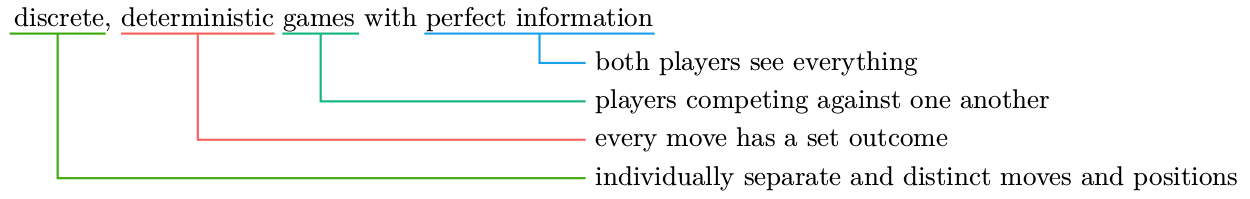
\includegraphics[width=\textwidth]{fig/game.png}
    \end{figure}
\end{frame}


\begin{frame}
    \frametitle{Monte Carlo Tree Search}
    % 蒙特卡罗树搜索是一种基于树数据结构、能权衡探索与利用、在搜索空间巨大仍然比较有效的的搜索算法。
    \begin{block}{Definition}
    which is a heuristic search algorithm for some kinds of decision processes, typically move planning in combinatorial games. It combines the generality of random simulation with the precision of tree search.
    \end{block}

    MCTS deals with large trees effectively by sampling many paths down the game tree. This means it repeatedly goes down many, but not all. As it tries more paths, it gains better estimates for which paths are good. Each one of these sample trials is called a Monte Carlo simulation.

    \begin{columns}
    \begin{column}{0.4\textwidth}
        The process can be broken down into the four phases
    \end{column}

    \begin{column}{0.4\textwidth}
    \begin{itemize}
        \reditem Selection
        \reditem Expansion
        \reditem Simulation
        \reditem Backpropagation
    \end{itemize}
    \end{column}
    \end{columns}
\end{frame}


\begin{frame}
    \frametitle{Basic Algorithm}

    \begin{figure}
        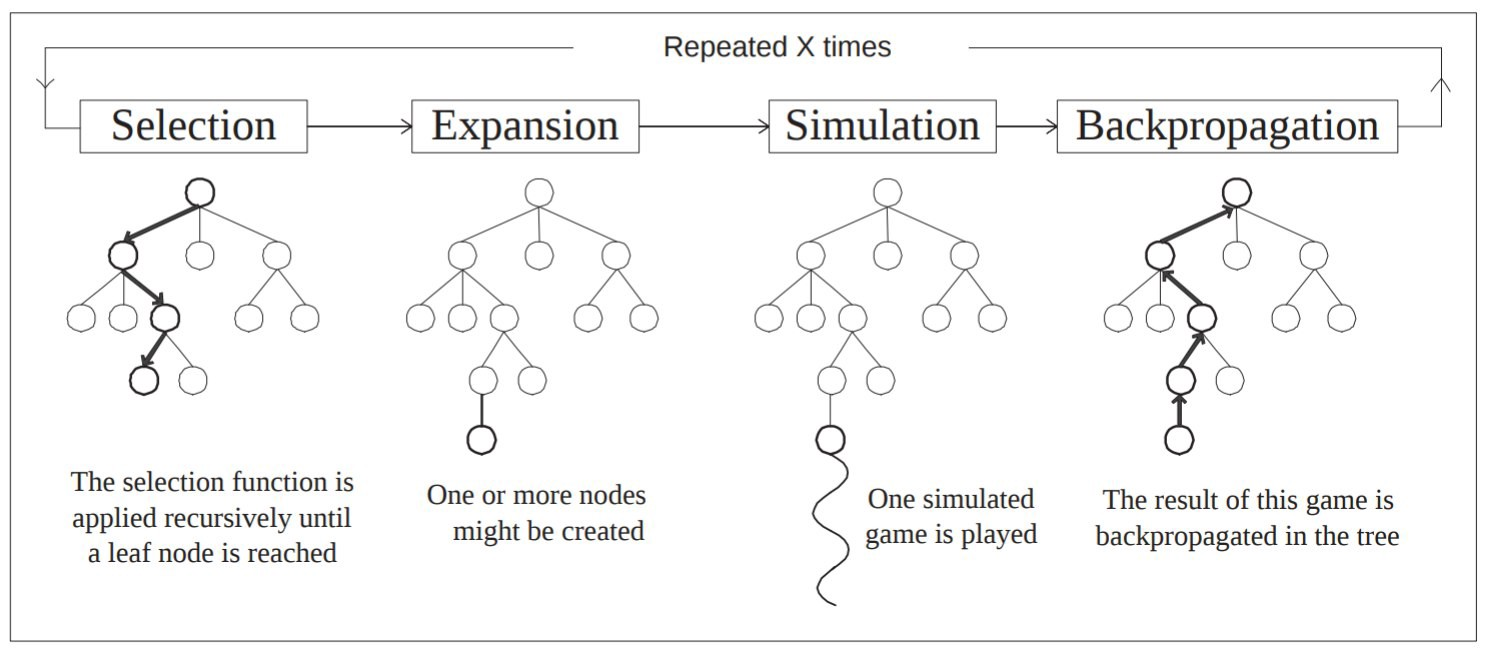
\includegraphics[width=\textwidth]{fig/mcts_process.png}
        \caption{Monte Carlo tree search procedure, diagram from Chaslot (2006)}
    \end{figure}
\end{frame}

\begin{frame}
    \frametitle{MCTS in Detail}

    \center \large \textbf{Take a game of tic-tac-toe as example}
    \\[2em]

    \begin{columns}
        \begin{column}{0.05\textwidth}\end{column}
        \begin{column}{0.55\textwidth}
            \begin{itemize}
                \reditem initial state $s_0$ 
                \reditem a set of actions $\mathcal{A}$
                \reditem terminal state: $\{win, loss, tie\}$
                \reditem score: $\{+1, -1, 0\}$
            \end{itemize}
        \end{column}

        \begin{column}{0.4\textwidth}
            \begin{figure}
                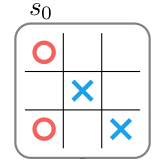
\includegraphics[width=0.6\textwidth]{fig/s0.png}
            \end{figure}
        \end{column}

    \end{columns}

\end{frame}

\begin{frame}
    \frametitle{Phase 2: Expansion}
    % If L is a not a terminal node (i.e. it does not end the game) then create one or more child nodes and select one C.
    \begin{figure}
        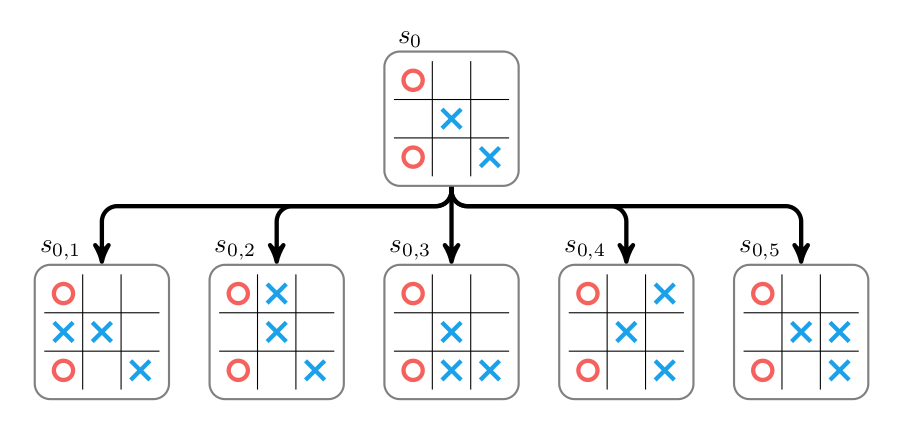
\includegraphics[width=\textwidth]{fig/mcts_expansion.png}
        \caption{This node is expanded by trying every action $a \in \mathcal{A}$}
    \end{figure}
\end{frame}

\begin{frame}
    \frametitle{Phase 3: Simulation}
    % Run a simulated playout from C until a result is achieved.
    \begin{figure}
        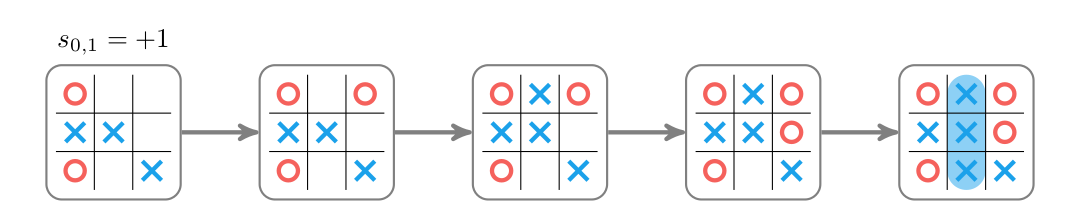
\includegraphics[width=\textwidth]{fig/mcts_simulation.png}
        \caption{The child node is rolled out by randomly taking moves from the child state until a win, loss, or tie is reached}
    \end{figure}
\end{frame}

\begin{frame}
    \frametitle{Phase 4: Backpropagation}
    % Update the current move sequence with the simulation result.
    \begin{figure}
        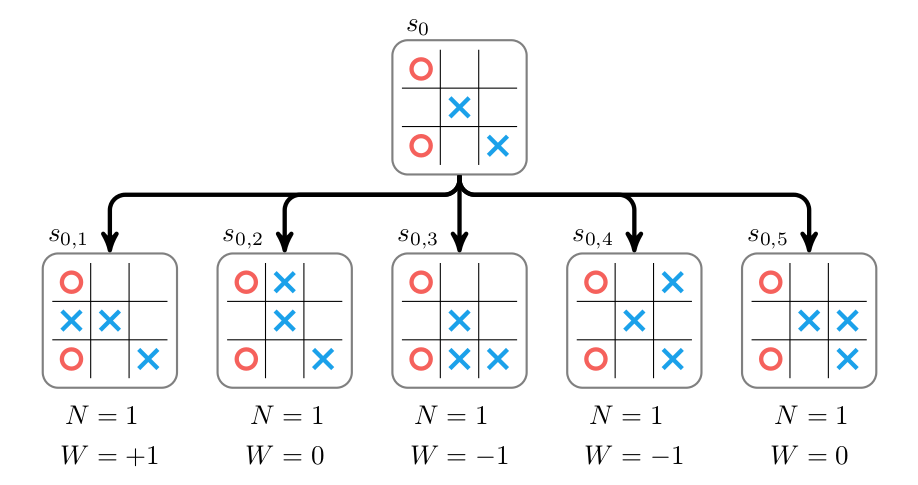
\includegraphics[width=\textwidth]{fig/expanded_tree.png}
        \caption{The expanded tree with approximate values for each child node}
    \end{figure}
\end{frame}

\begin{frame}
    \frametitle{Phase 4: Backpropagation}

    \begin{figure}
        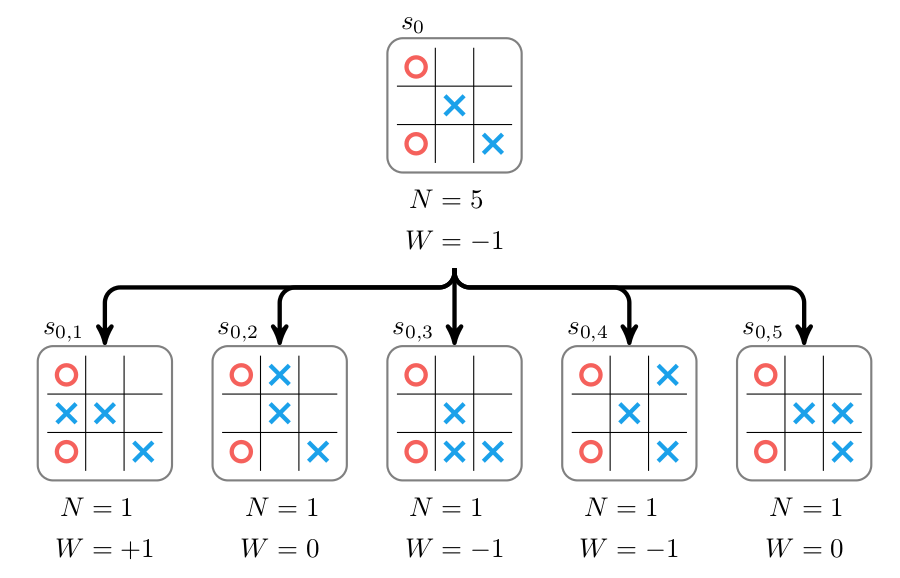
\includegraphics[width=0.9\textwidth]{fig/mcts_backpropagation.png}
        \caption{The information from the child nodes is then propagated back up the tree by increasing the parent's value and visit count}
    \end{figure}
\end{frame}

\begin{frame}
    \frametitle{Credit Assignment Problem} % 贡献度分配问题
    % 贡献度分配问题即一个系统中不同的组件 (components)对最终系 统输出结果的贡献或影响。
    % 强化学习中的关键问题也是贡献度分配问题 [Minsky, 1963],每一个动作并不能直接得到监督信息,需要通过整个模型的最终监督信 息(奖励)得到,并且有一定的延时性。
    Monte Carlo tree search does not expand all leaf nodes, as that would be very expensive. Instead, the selection process chooses nodes that strike a balance between being lucrative -- having \underline{high estimated values}, and being relatively unexplored -- having \underline{low visit counts}.
\end{frame}


\begin{frame}
    \frametitle{UCT Score}

    A leaf node is selected by traversing down the tree from the root node, always choosing the child $i$ with the highest upper confidence tree (UCT) score:

    $$
    U_i = \frac{W_i}{N_i} + c\sqrt{\frac{\ln N_p}{N_i}}
    $$

    where \\
    \hspace{1em} $W_i$ is the accumulated value of the $i$th child \\
    \hspace{1em} $N_i$ is the visit count for $i$th child \\
    \hspace{1em} $N_p$ is the number of visit counts for the parent node \\
    \hspace{1em} The parameter $c \ge 0$ controls the tradeoff between choosing lucrative nodes (low $c$) and exploring nodes with low visit counts (high $c$)
\end{frame}

\begin{frame}
    \frametitle{Phase 1: Selection}

    \begin{figure}
        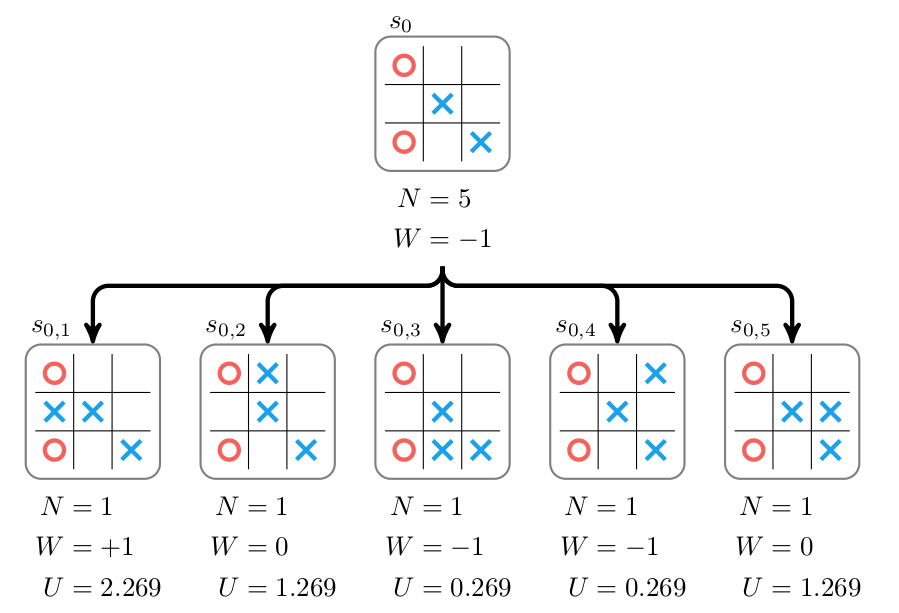
\includegraphics[width=0.9\textwidth]{fig/mcts_selection.png}
        \caption{The UCT scores for the tic-tac-toe tree with $c=1$}
    \end{figure}
\end{frame}

\begin{frame}
    \frametitle{Phase 2 to 4}

    \begin{figure}
        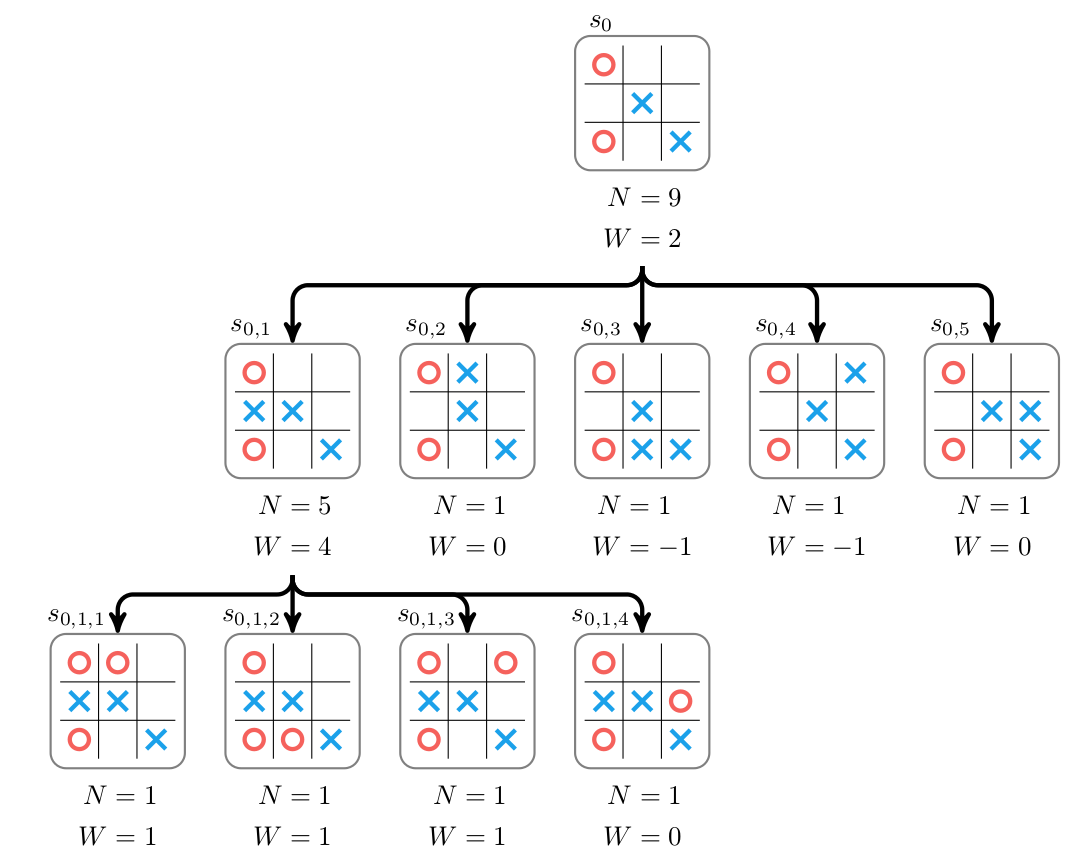
\includegraphics[width=0.75\textwidth]{fig/mcts_2_to_4.png}
        \caption{That node is expanded and the values are propagated back up}
    \end{figure}
\end{frame}

\begin{frame}
    \frametitle{Iterations}

    \begin{figure}
        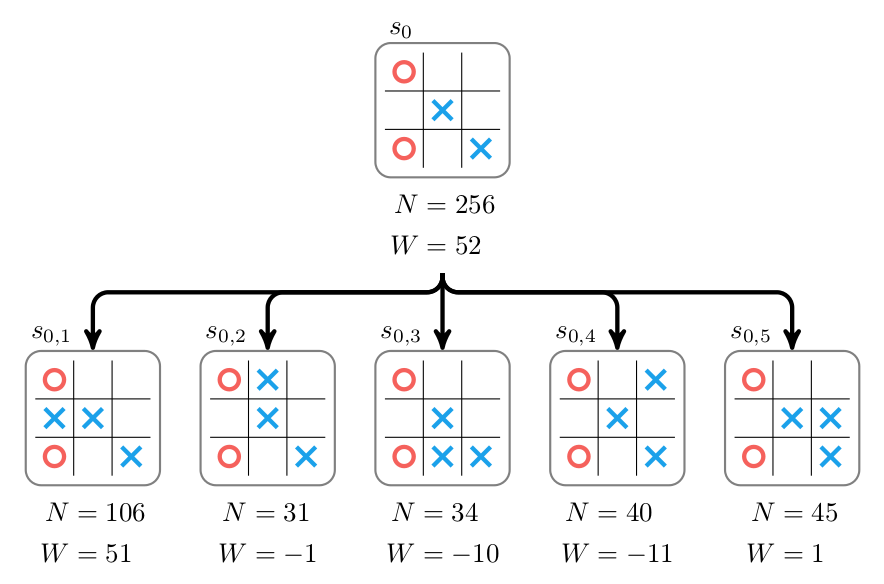
\includegraphics[width=0.9\textwidth]{fig/mcts_iterations.png}
        \caption{The tree is expanded and explore the possible moves, identifying the best move to take}
    \end{figure}
\end{frame}

\begin{frame}
    \frametitle{Efficiency Through Expert Policies}

    Games like chess and Go have very large branching factors. there are an estimated $10^{46}$ board states in chess, and Go played on a traditional 19x19 board has around $10^{170}$ (Tic-tac-toe only has 5478 states).
    \\[2em]
    Move evaluation with vanilla Monte Carlo tree search just isn't efficient enough.
    \\[2em]
    Suppose we have an expert policy $\pi$ that, for a given state $s$, tells us how likely an expert-level player is to make each possible action.
\end{frame}

\begin{frame}
    \frametitle{Expert Policies}

    \begin{figure}
        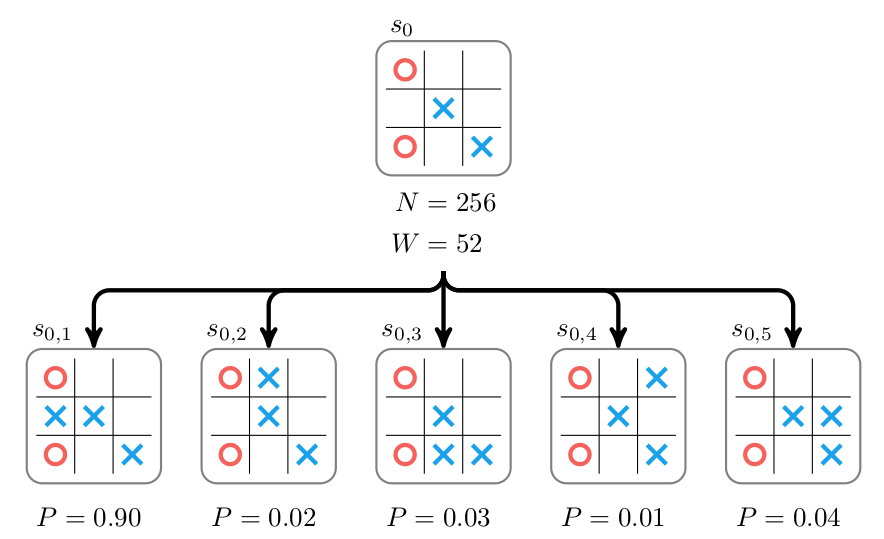
\includegraphics[width=0.9\textwidth]{fig/expert_policies.png}
        \caption{$P_i=\pi(a_i | s_0)$ is the probability of choosing the $i$th action $a_i$ given the root state $s_0$}
    \end{figure}
\end{frame}

\begin{frame}
    \frametitle{Expert Policies}
    A modified form of Monte Carlo tree search will store the probability of each node according to the policy, and this probability is used to adjust the node's score during selection.
    \\[2em]
    The probabilistic upper confidence tree score used by DeepMind is:
    $$
    U_i = \frac{W_i}{N_i} + cP_i\sqrt{\frac{\ln N_p}{1+N_i}}
    $$
    \\[2em]
    Now, node exploration is guided by the expert policy, biasing exploration towards moves the expert policy considers likely.
\end{frame}

\begin{frame}
    \frametitle{Efficiency Through Value Approximation}

    A second form of efficiency can be achieved by avoiding expensive and potentially inaccurate random rollouts.
    \\[1em]
    \begin{itemize}
        \reditem Use the expert policy from the previous section to guide the random rollout
        \reditem Avoid rollouts altogether, directly approximate the value of a state with a value approximator function $\hat{W}(x)$
        \\[2em]
    \end{itemize}
    

    $\hat{W}(x)$ takes a state and directly computes a value in $[-1, 1]$, without conducting rollouts.
\end{frame}

\begin{frame}
    \frametitle{The Alpha Zero Neural Net}

    Alpha Zero uses one neural network $f$ that takes in the game state and produces both the probabilities over the next move and the approximate state value:
    \\[.2em]
    $$
    f(s) \rightarrow [\vec P, W] 
    $$
    \\[1em]
    Leaves in the search tree are expanded by evaluating them with the neural network. Each child is initialized with $N=0$, $W=0$ and with $P$ corresponding to the prediction from the network. The value of the expanded node is set to the predicted value and this value is then backed up the tree.
\end{frame}

\begin{frame}
    \frametitle{The Alpha Zero Neural Net}

    \begin{figure}
        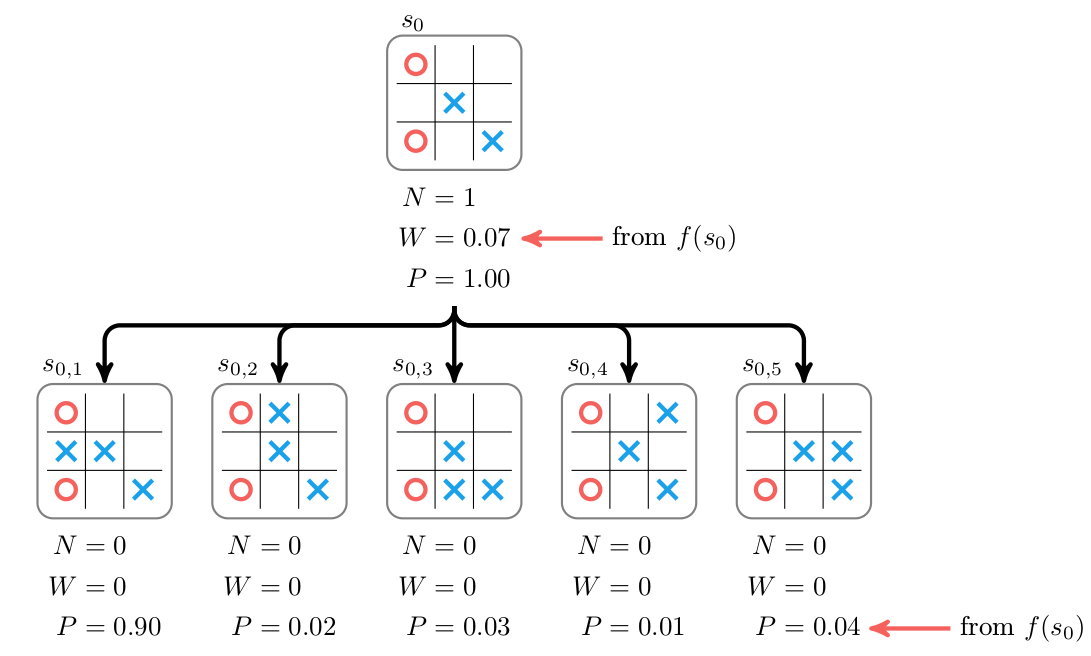
\includegraphics[width=\textwidth]{fig/alphagozero_mcts1.png}
    \end{figure}
\end{frame}

\begin{frame}
    \frametitle{The Alpha Zero Neural Net}

    \begin{figure}
        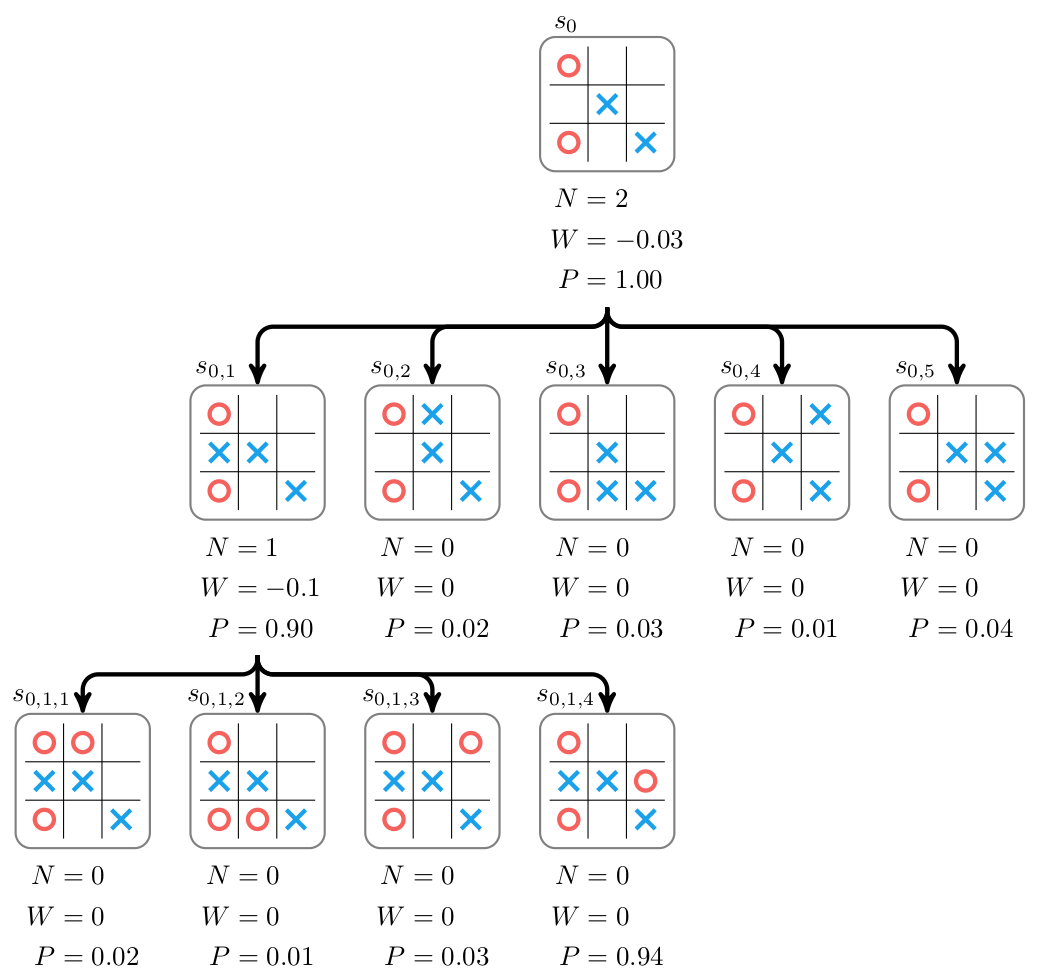
\includegraphics[height=0.85\textheight]{fig/alphagozero_mcts2.png}
    \end{figure}
\end{frame}

\begin{frame}
    \frametitle{The Alpha Zero Neural Net}
    The core idea of the Alpha Zero algorithm is that the predictions of the neural network can be improved, and the play generated by Monte Carlo tree search can be used to provide the training data.
    \\[1em]
    The \underline{policy portion} of the neural network is improved by training the predicted probabilities $P$ for $s_0$ to match the improved probability $\pi$ obtained from running Monte Carlo tree on $s_0$:
    $$
    \pi_i = N_i^{1/\tau}
    $$

    The \underline{value portion} of the neural network is improved by training the predicted value to match the eventual win/loss/tie result of the game, $Z$.
\end{frame}

\begin{frame}
    \frametitle{The Loss Function}

    The Alpha Zero neural network's loss function is:
    $$
    (w-z)^2 + \bm{\pi}^\intercal \ln \mathbf{p} + \lambda ||\bm{\theta}||_2^2
    $$
    where \\
    \hspace{2em} $(w-z)^2$ is the value loss \\
    \hspace{2em} $\bm{\pi}^\intercal \ln \mathbf{p}$ is the policy loss \\
    \hspace{2em} $\lambda ||\bm{\theta}||_2^2$ is an extra regularization term with parameter $\lambda \ge 0$ and $\theta$ represents the parameters in the neural network.
\end{frame}


\section{AlphaGo Zero}
\begin{frame}
    \center \huge \textbf{AlphaGo Zero}
\end{frame}

\begin{frame}
    \frametitle{The Deep Neural Network Architecture}

    The network learns 'tabula rasa'(from a blank slate)
    \\[.5em]
    At no point is the network trained using human knowledge or expert moves
    \\[.5em]
    \begin{figure}
        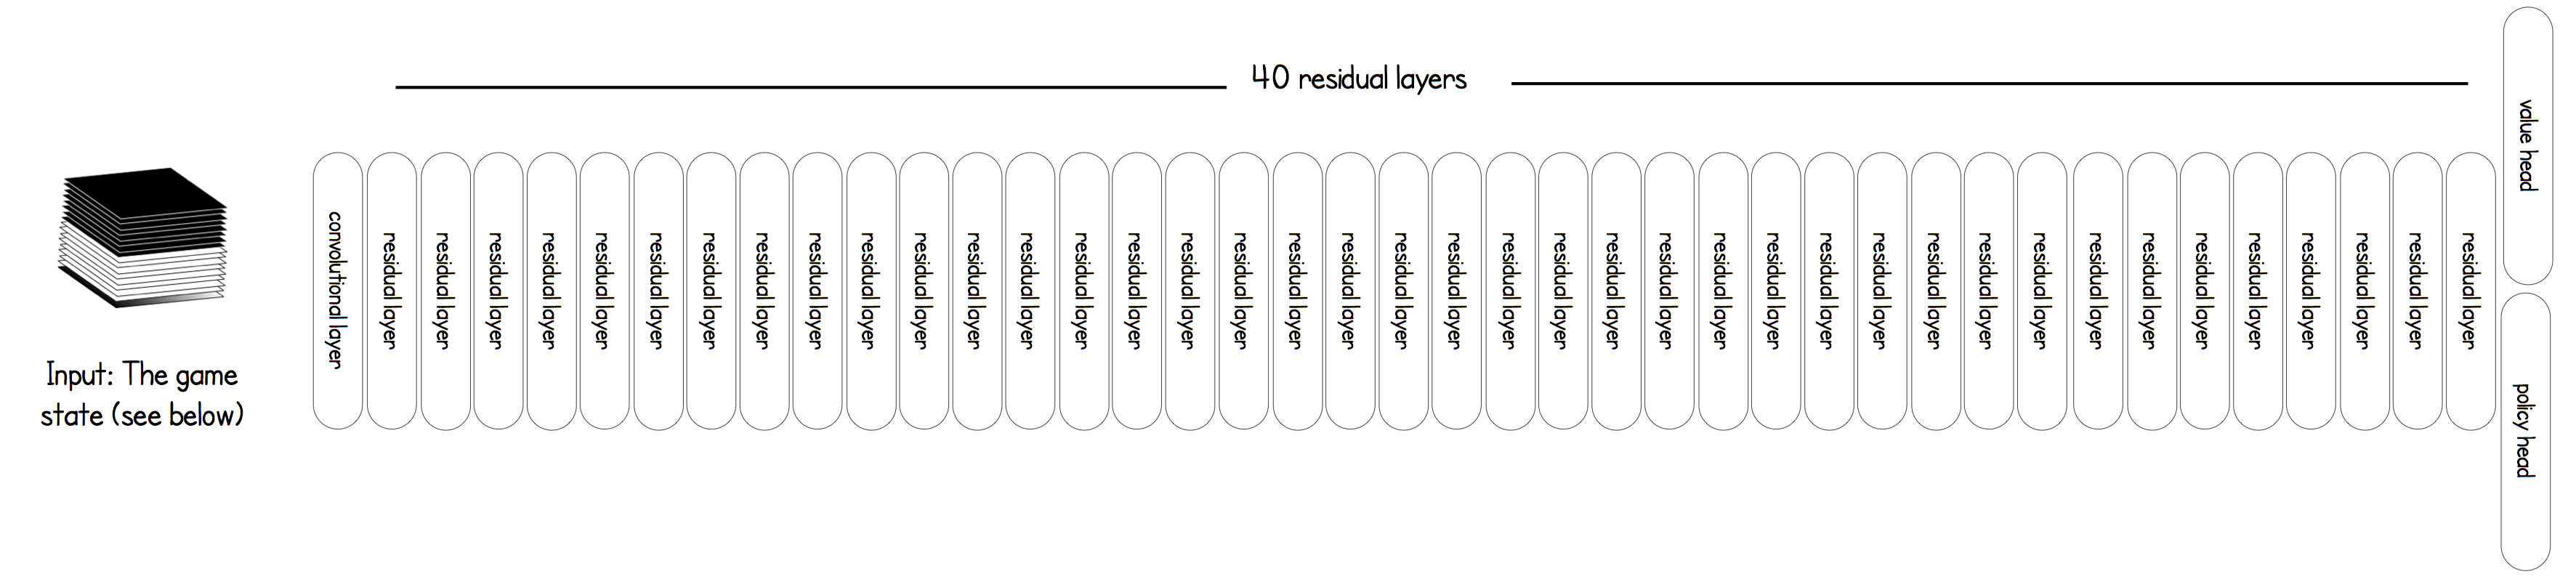
\includegraphics[width=\textwidth]{fig/neural_netwrok_architecture.png}
    \end{figure}
\end{frame}

\begin{frame}
    \frametitle{What Is A Game State}

    \begin{figure}
        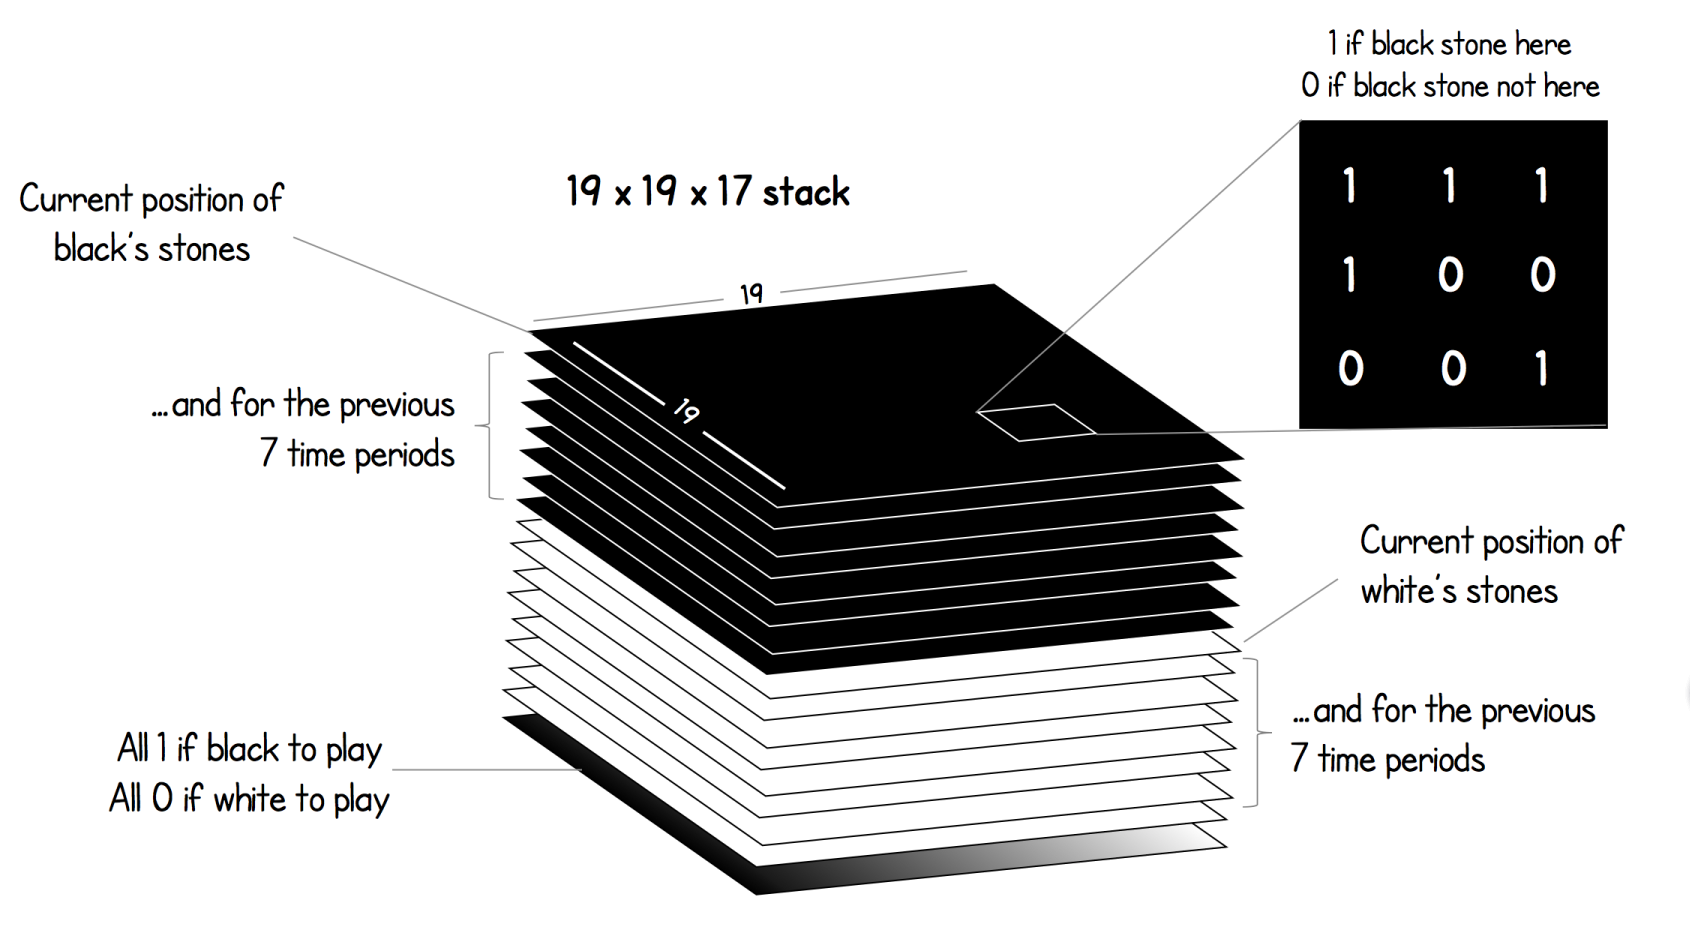
\includegraphics[width=\textwidth]{fig/game_state.png}
        \caption{The stack is the input to the deep neural network}
    \end{figure}

\end{frame}

\begin{frame}
    \frametitle{Convolutional Layer}

    \begin{figure}
        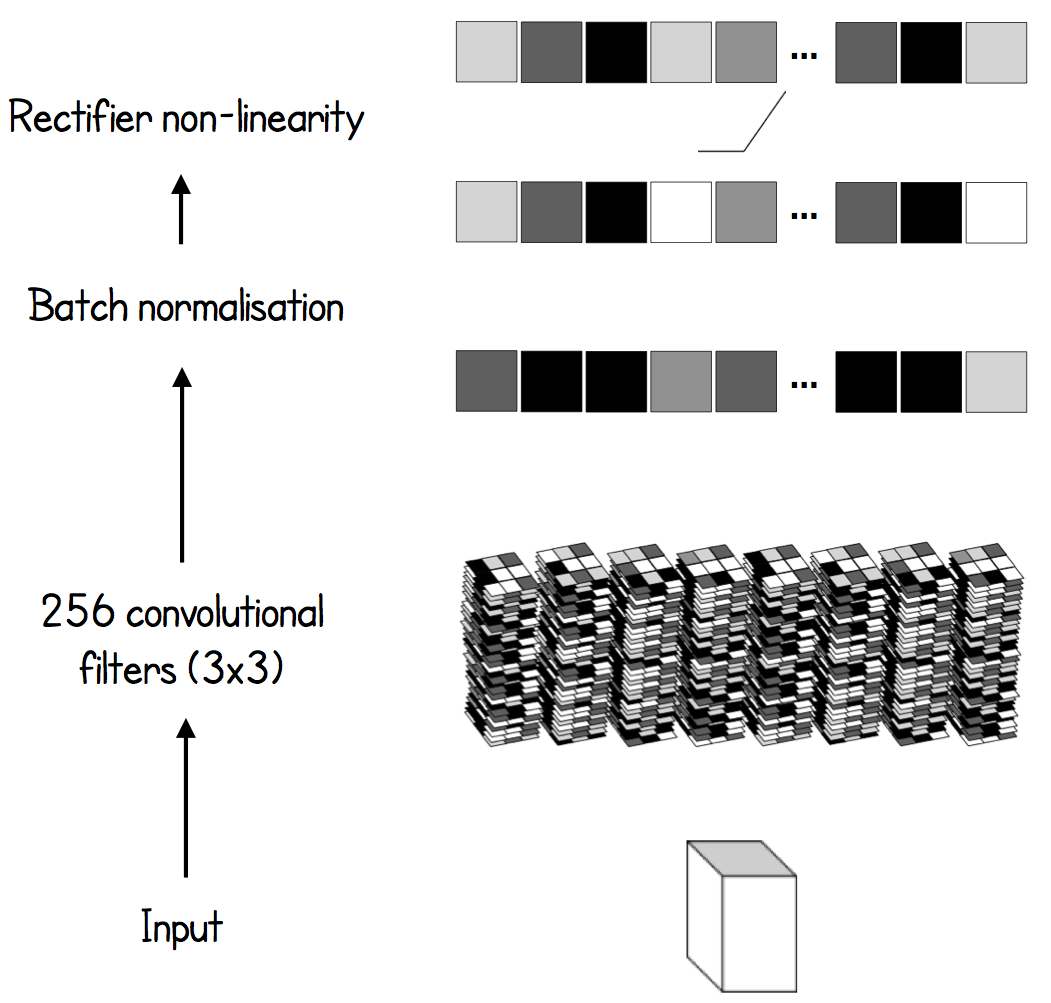
\includegraphics[height=0.9\textheight]{fig/convolutional_layer.png}
    \end{figure}
\end{frame}

\begin{frame}
    \frametitle{Residual Layer}

    \begin{figure}
        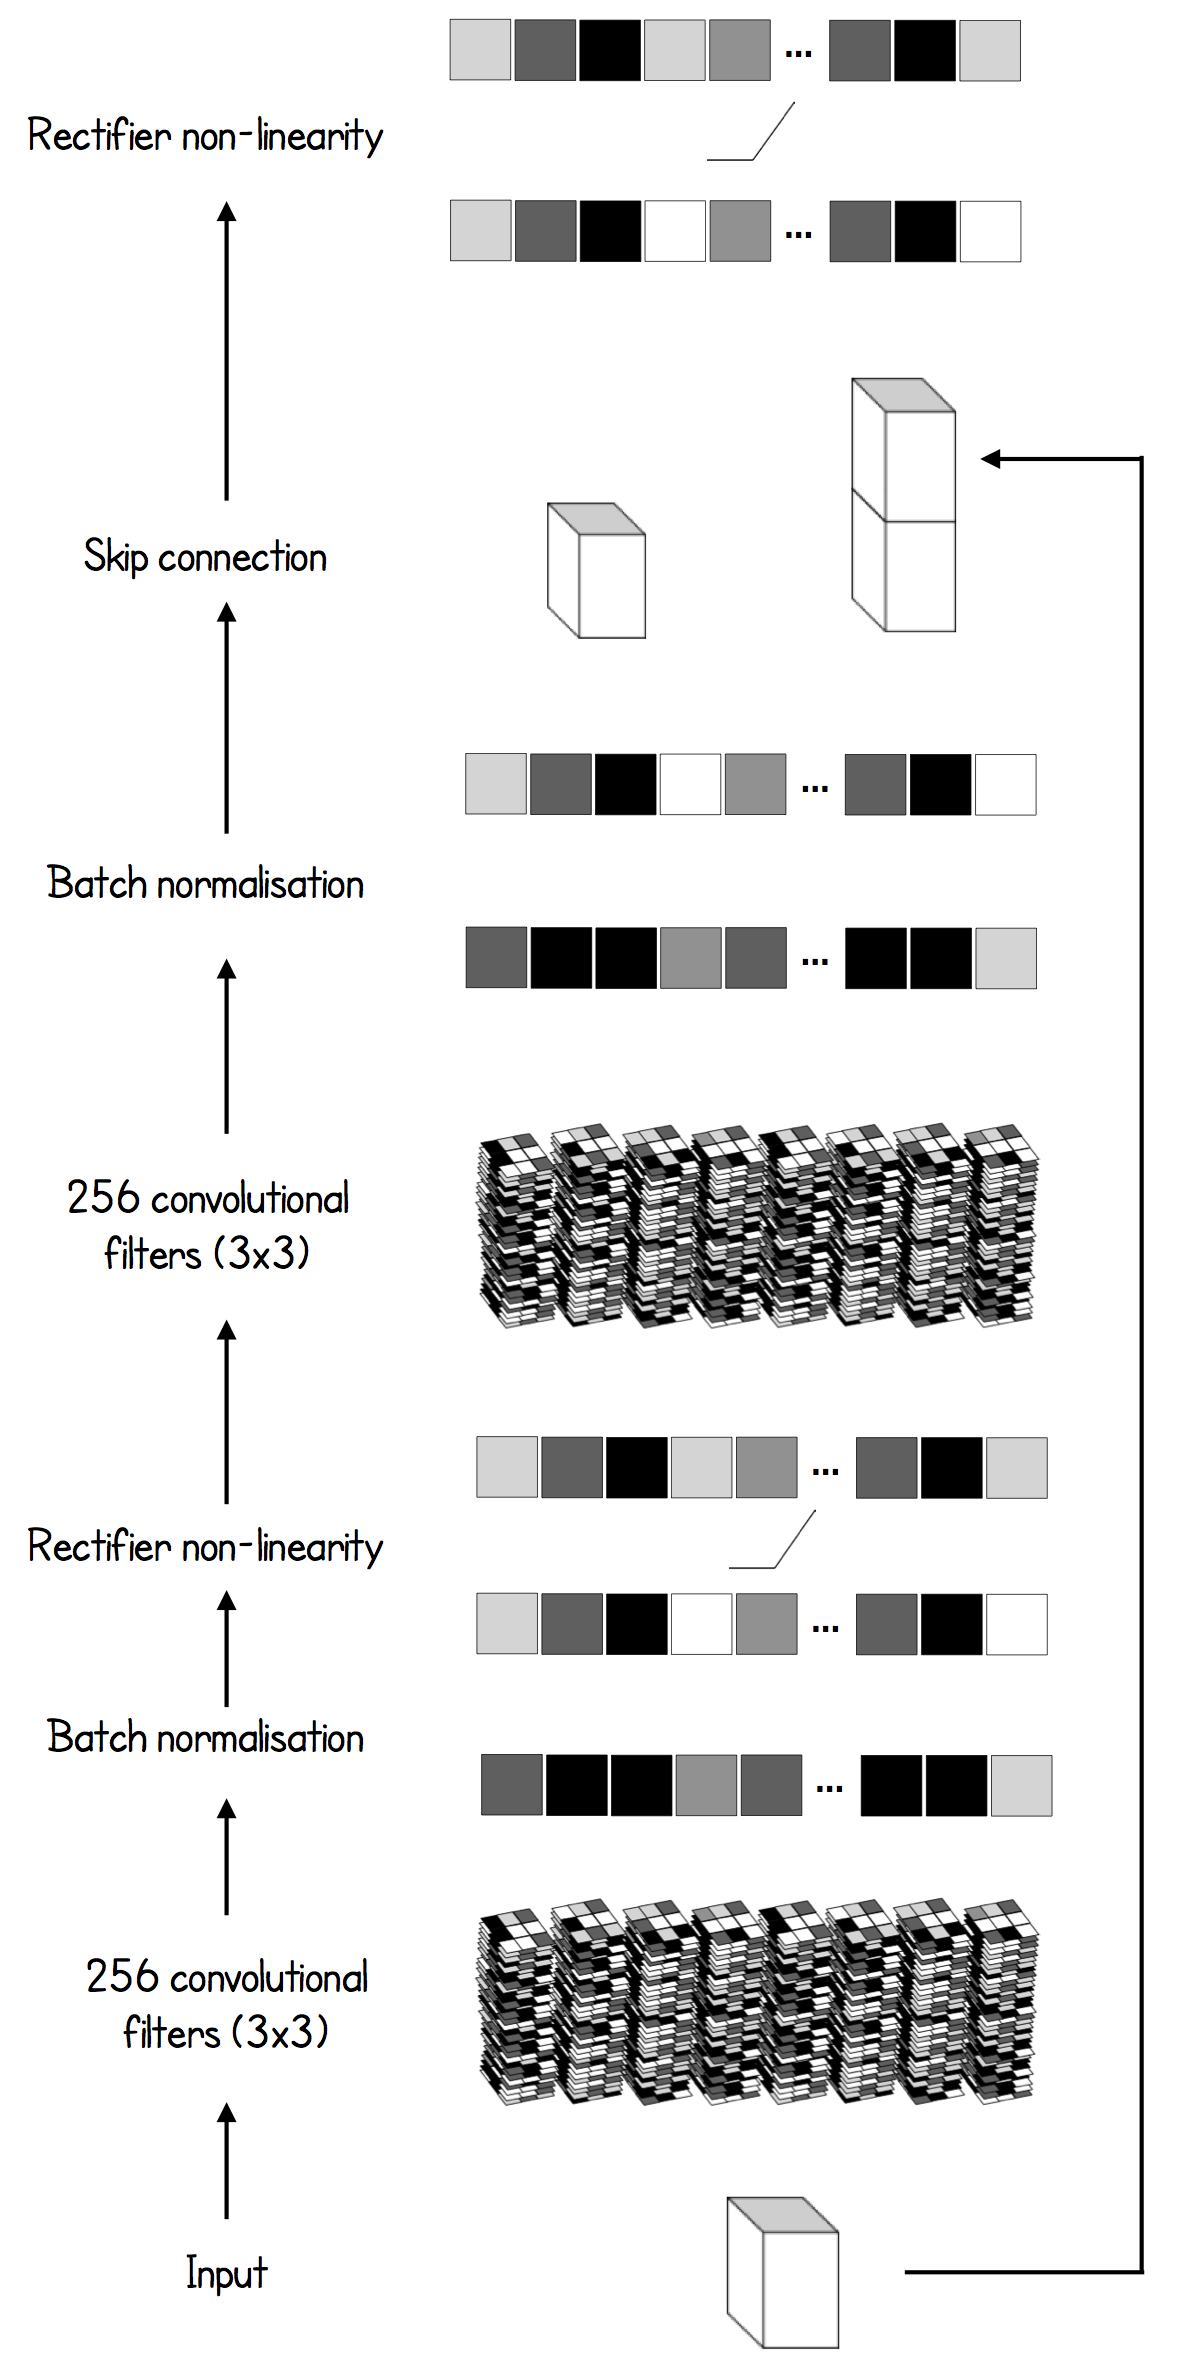
\includegraphics[height=0.9\textheight]{fig/residual_layer.png}
    \end{figure}
\end{frame}

\begin{frame}
    \frametitle{The Value Head}

    \begin{figure}
        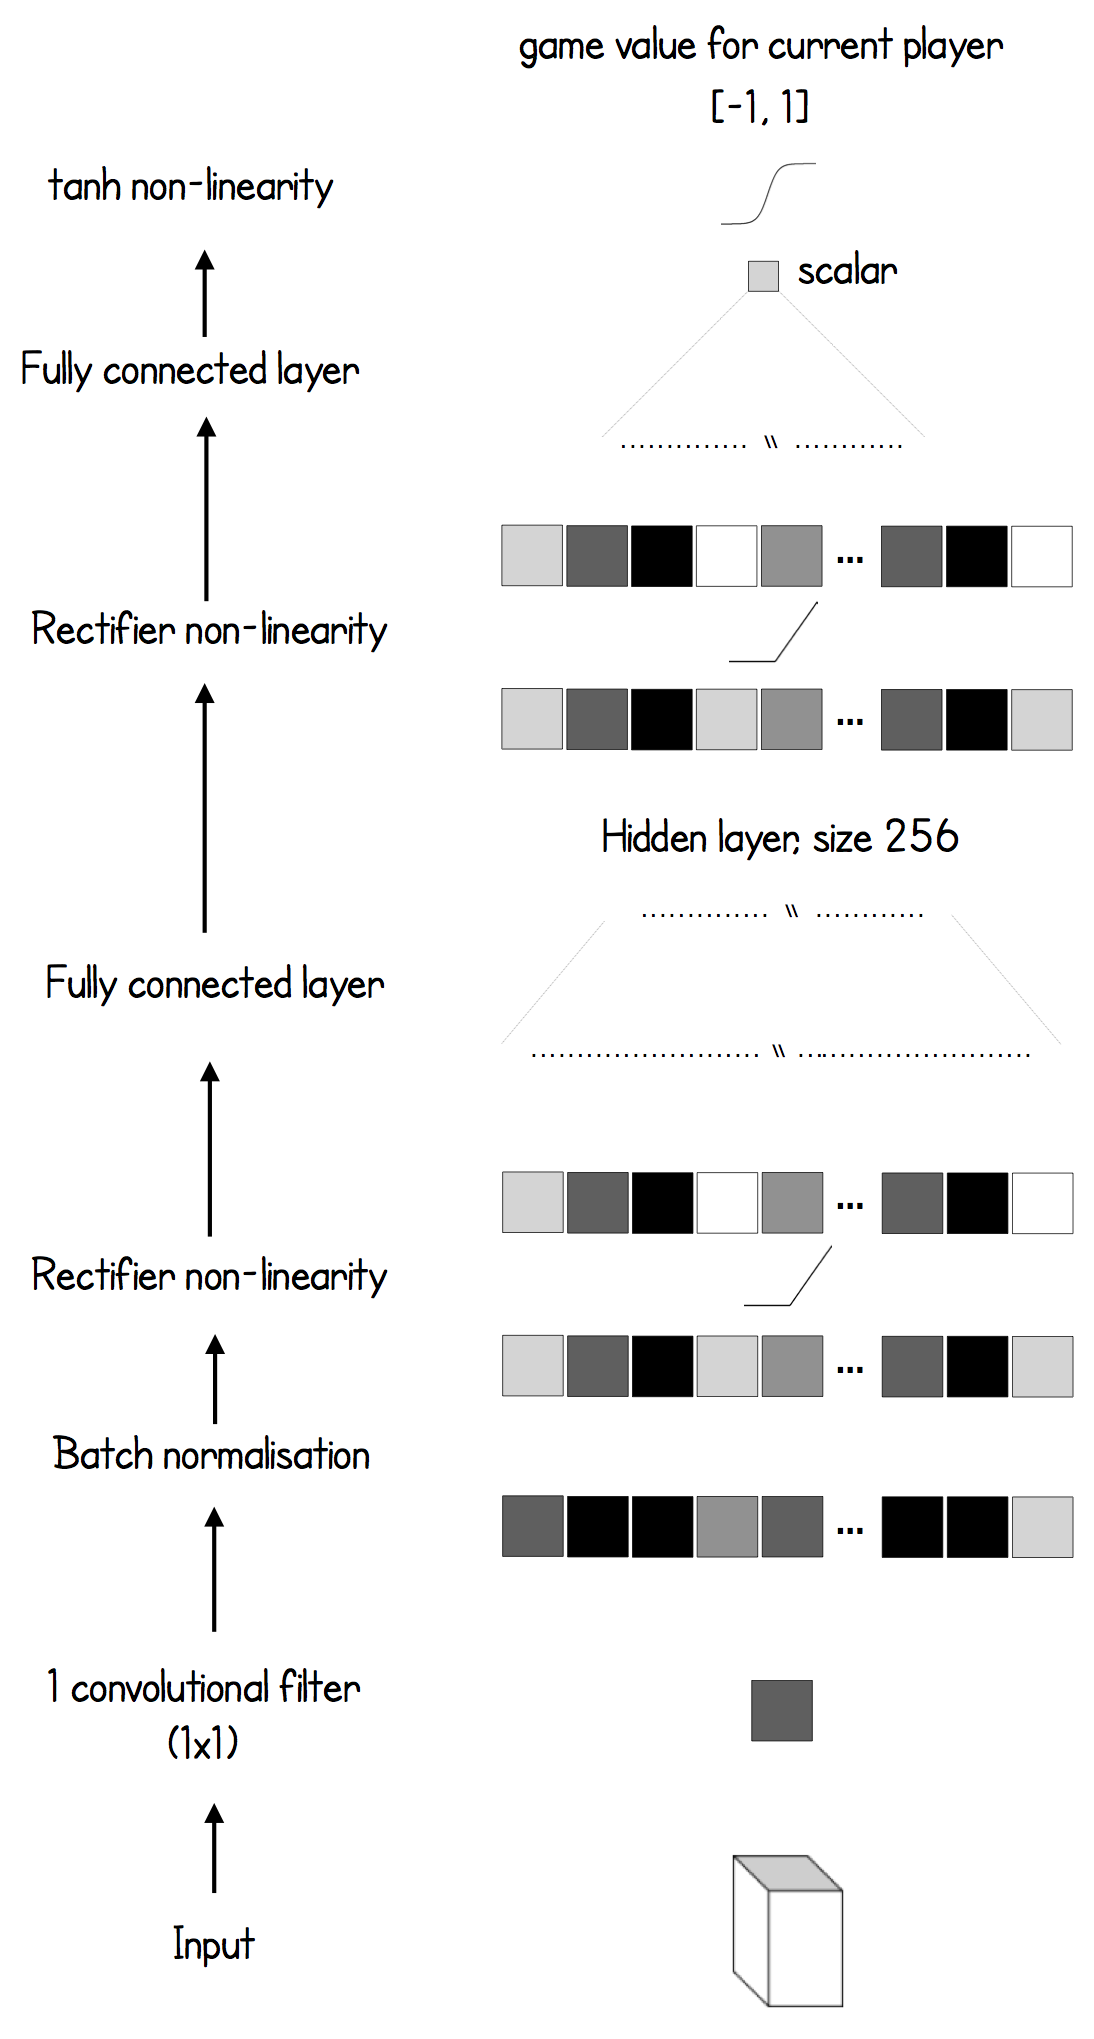
\includegraphics[height=0.9\textheight]{fig/the_value_head.png}
    \end{figure}
\end{frame}

\begin{frame}
    \frametitle{The Policy Head}

    \begin{figure}
        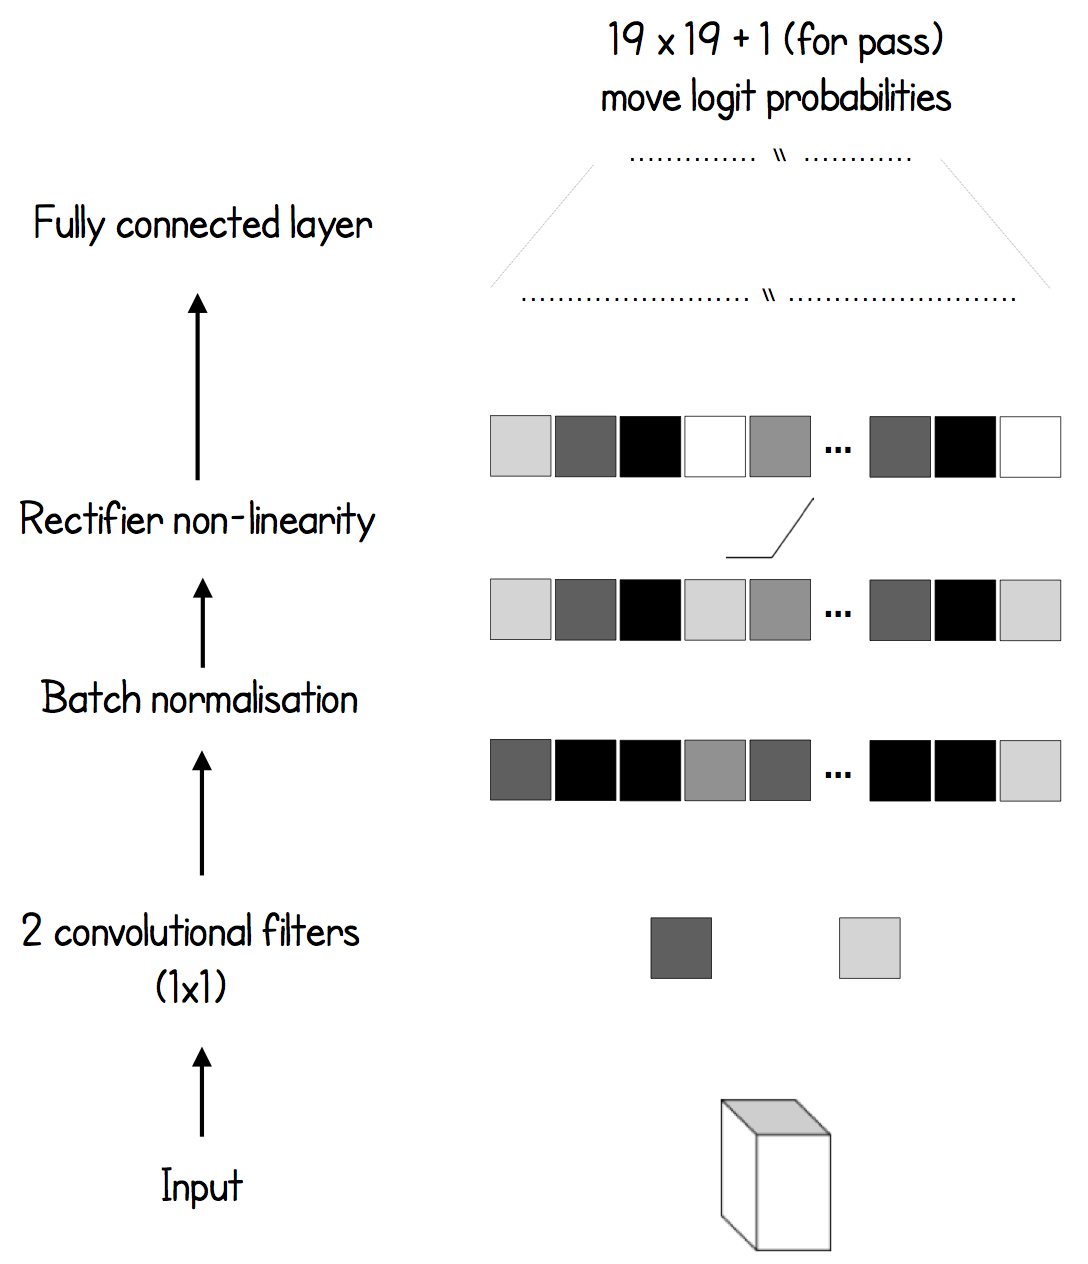
\includegraphics[height=0.9\textheight]{fig/the_policy_head.png}
    \end{figure}
\end{frame}

\begin{frame}
    \frametitle{How AlphaGo Zero Chooses Its Next Move}

    \begin{figure}
        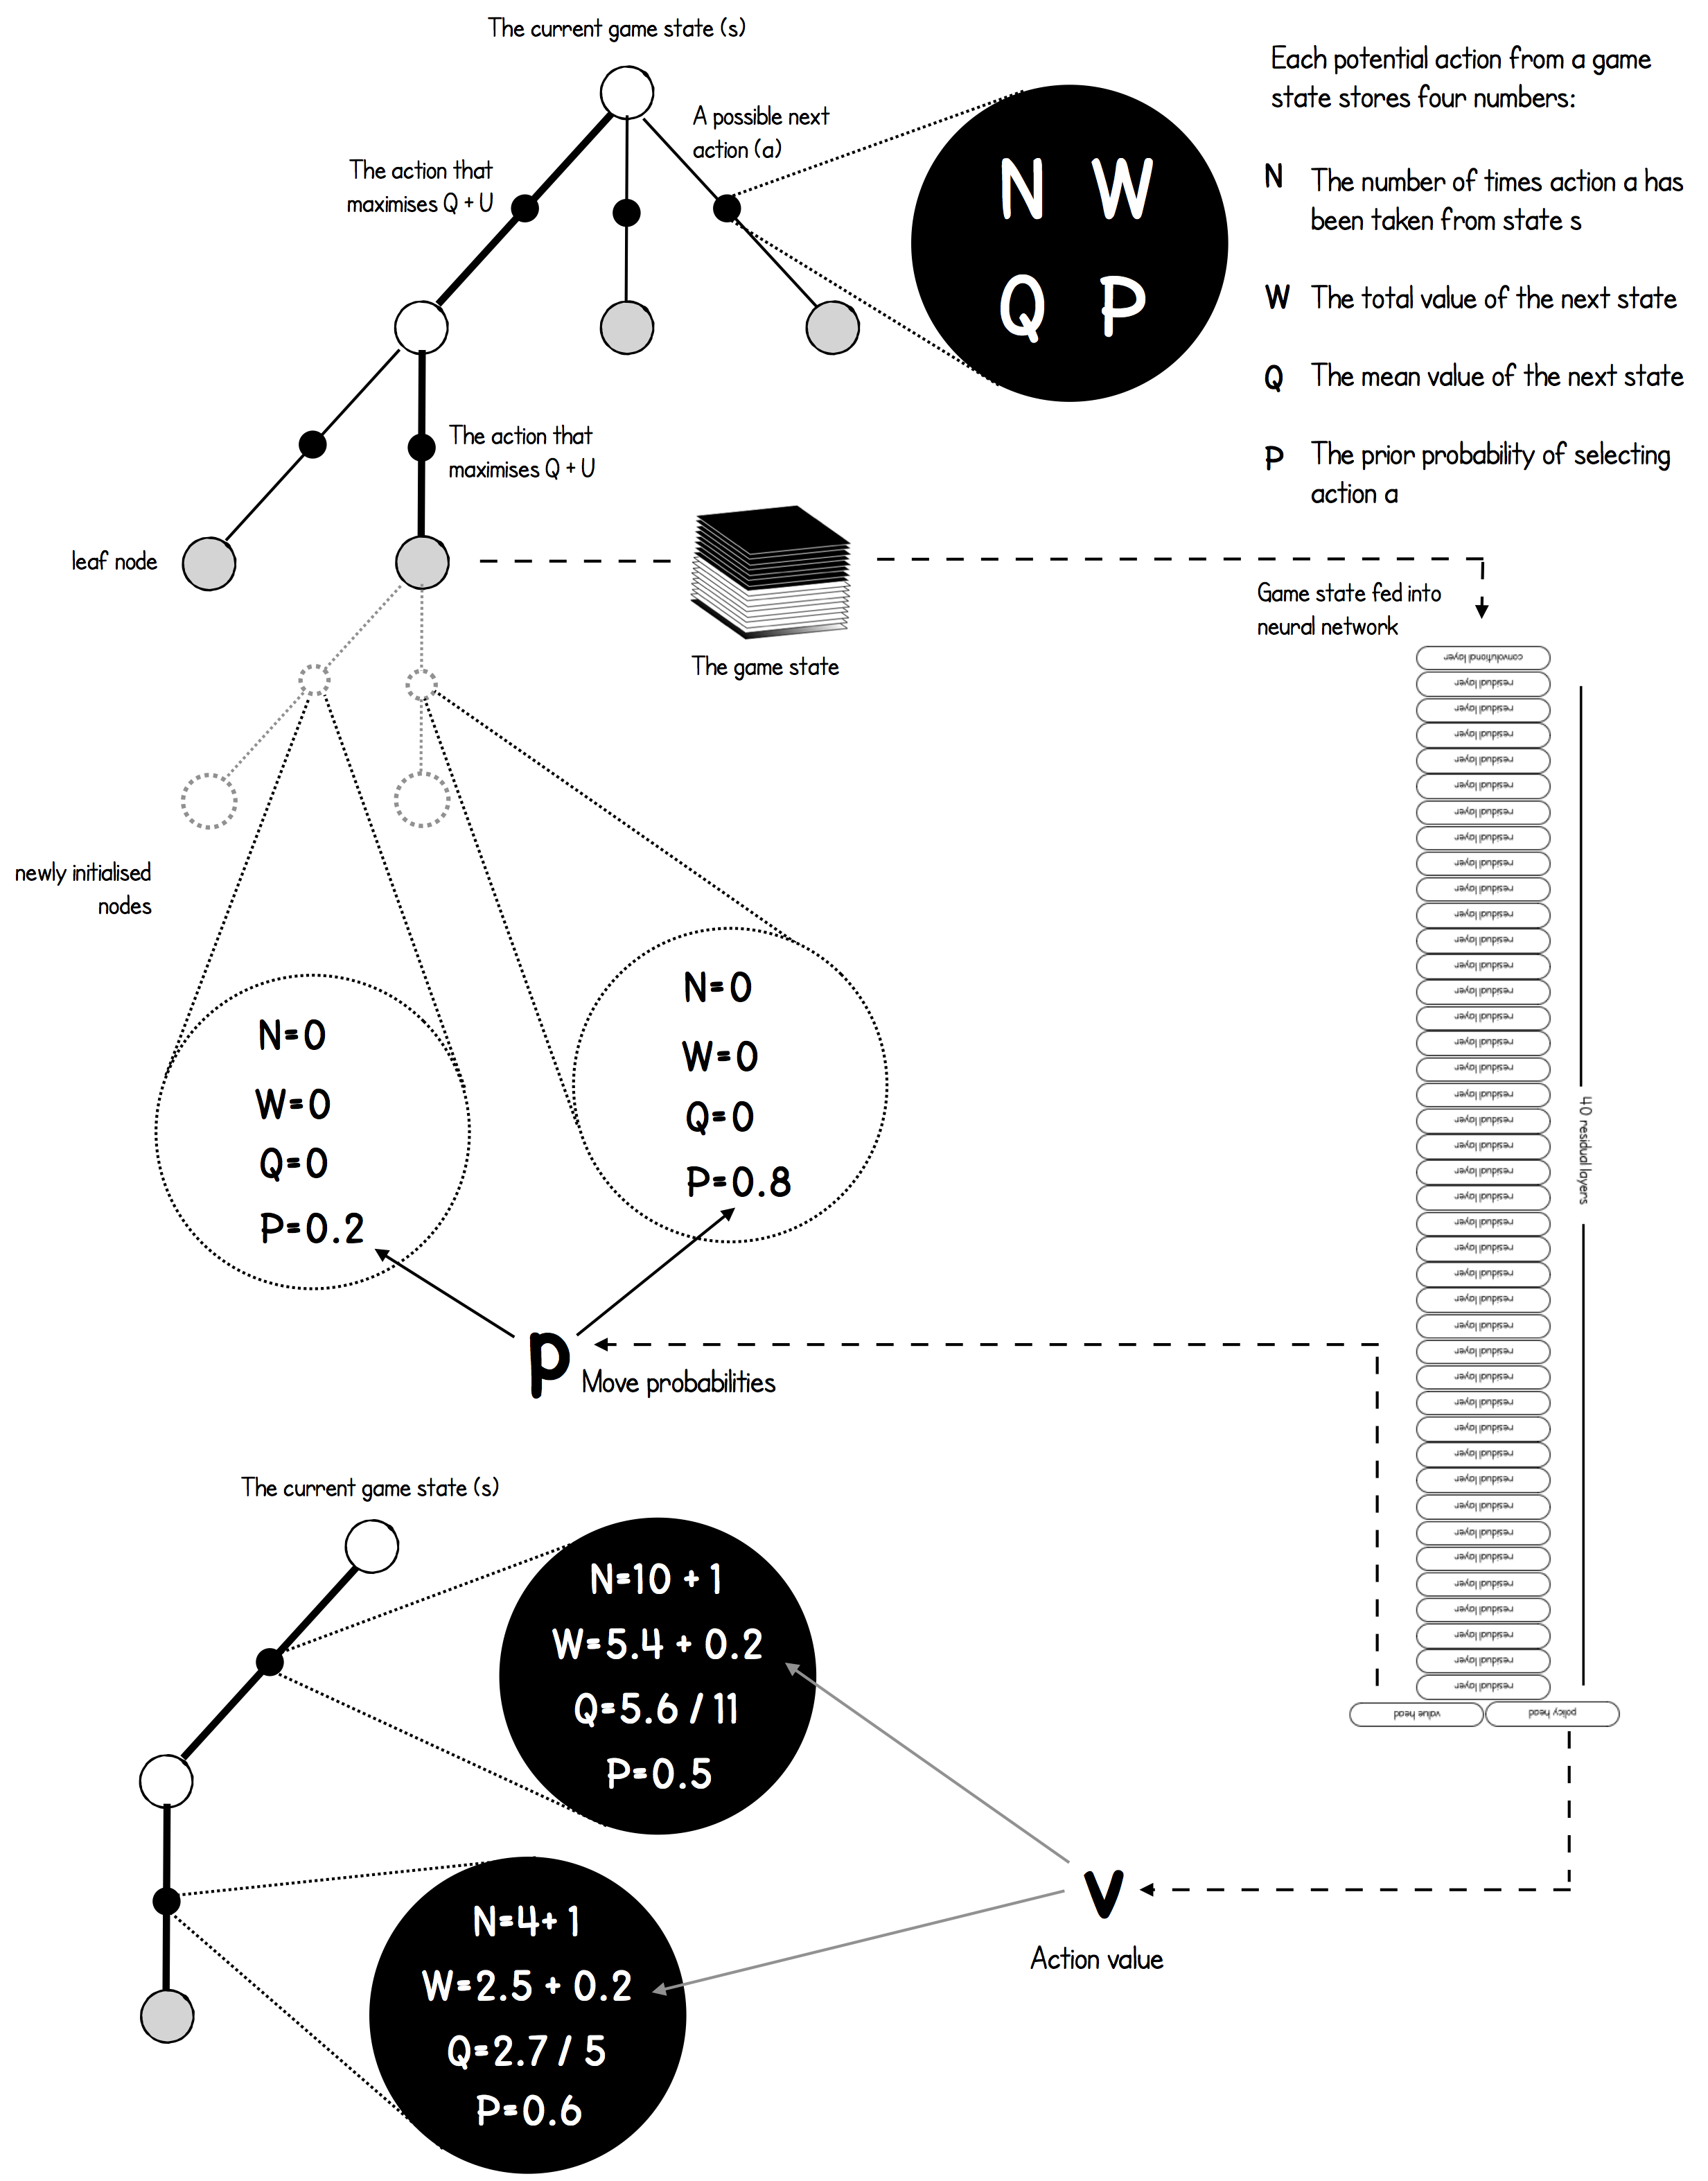
\includegraphics[height=0.9\textheight]{fig/alpha_mcts0.png}
    \end{figure}
\end{frame}

\begin{frame}
    \frametitle{How AlphaGo Zero Chooses Its Next Move}

    \begin{figure}
        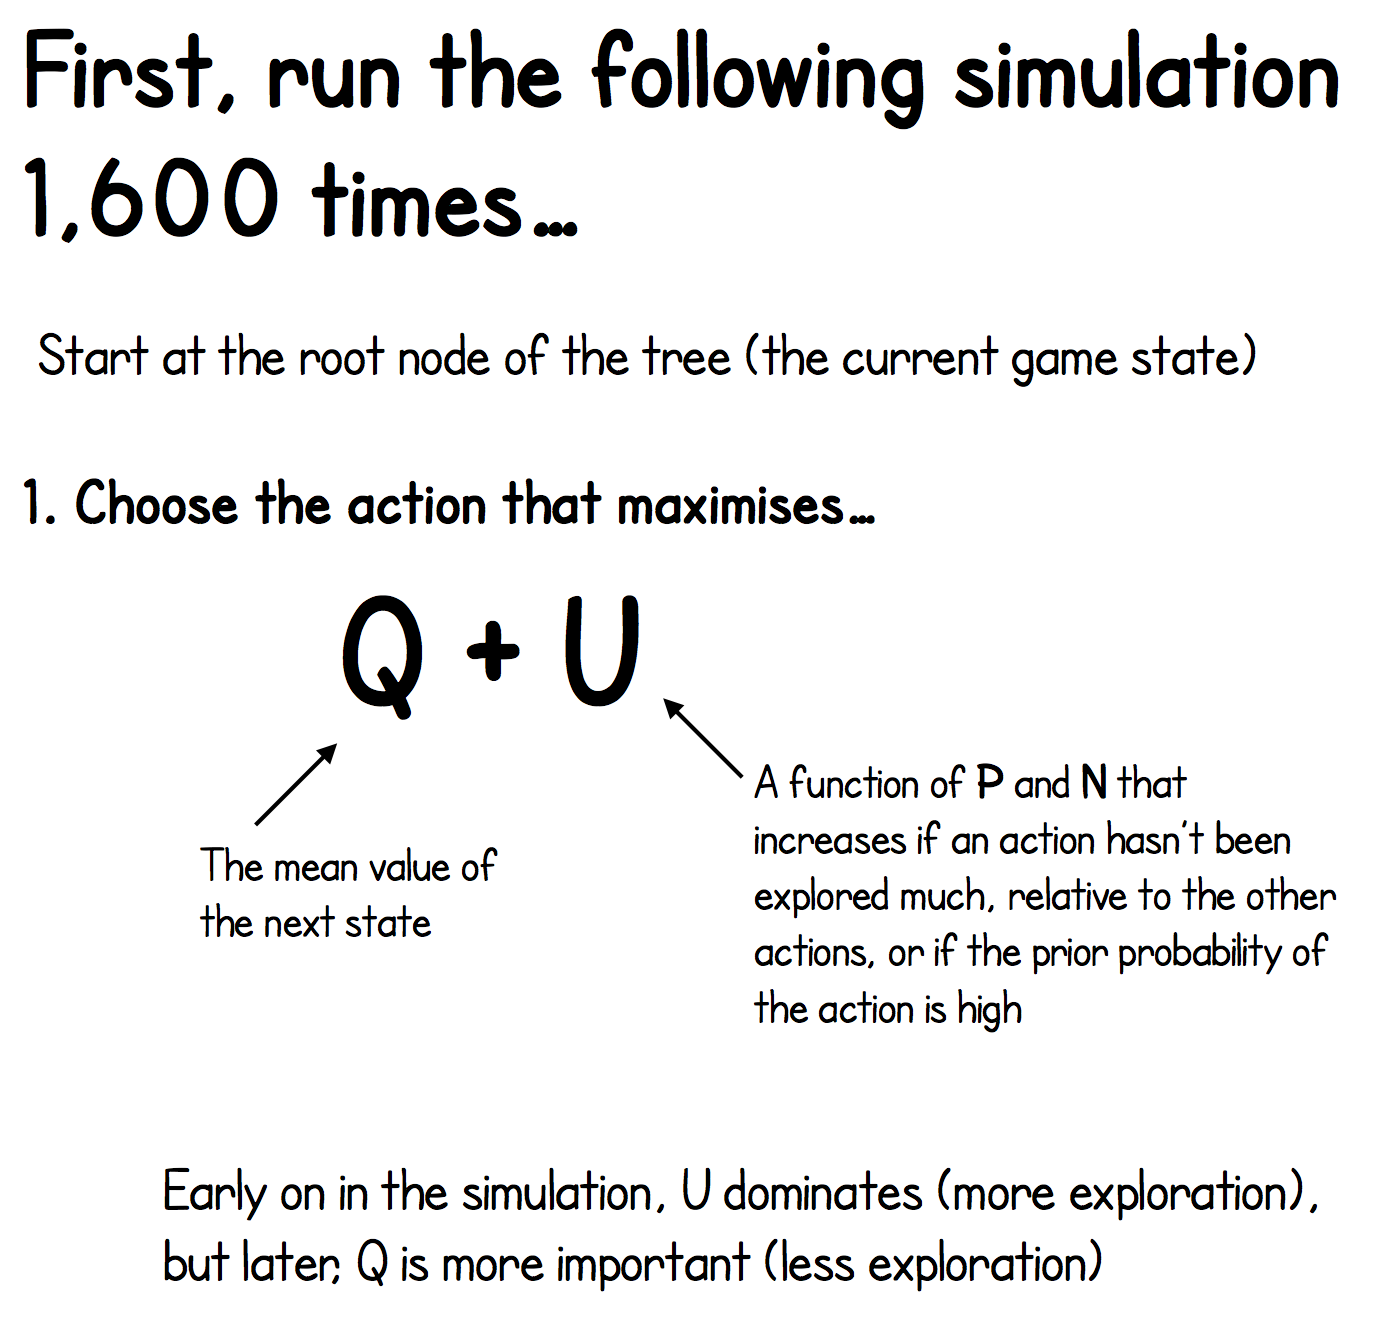
\includegraphics[height=0.8\textheight]{fig/alpha_mcts1.png}
    \end{figure}
\end{frame}

\begin{frame}
    \frametitle{How AlphaGo Zero Chooses Its Next Move}

    \begin{figure}
        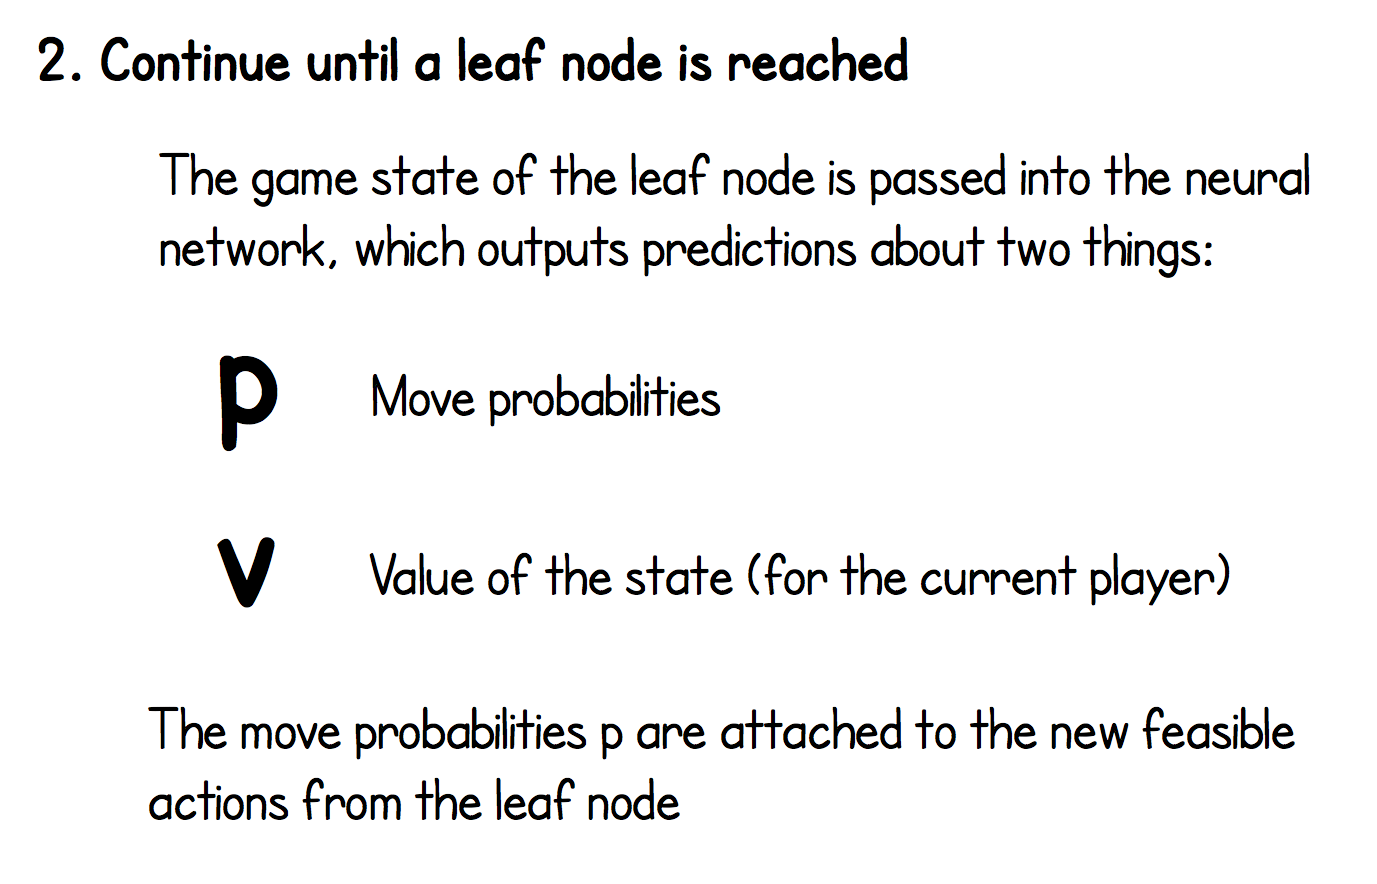
\includegraphics[height=0.7\textheight]{fig/alpha_mcts2.png}
    \end{figure}
\end{frame}

\begin{frame}
    \frametitle{How AlphaGo Zero Chooses Its Next Move}

    \begin{figure}
        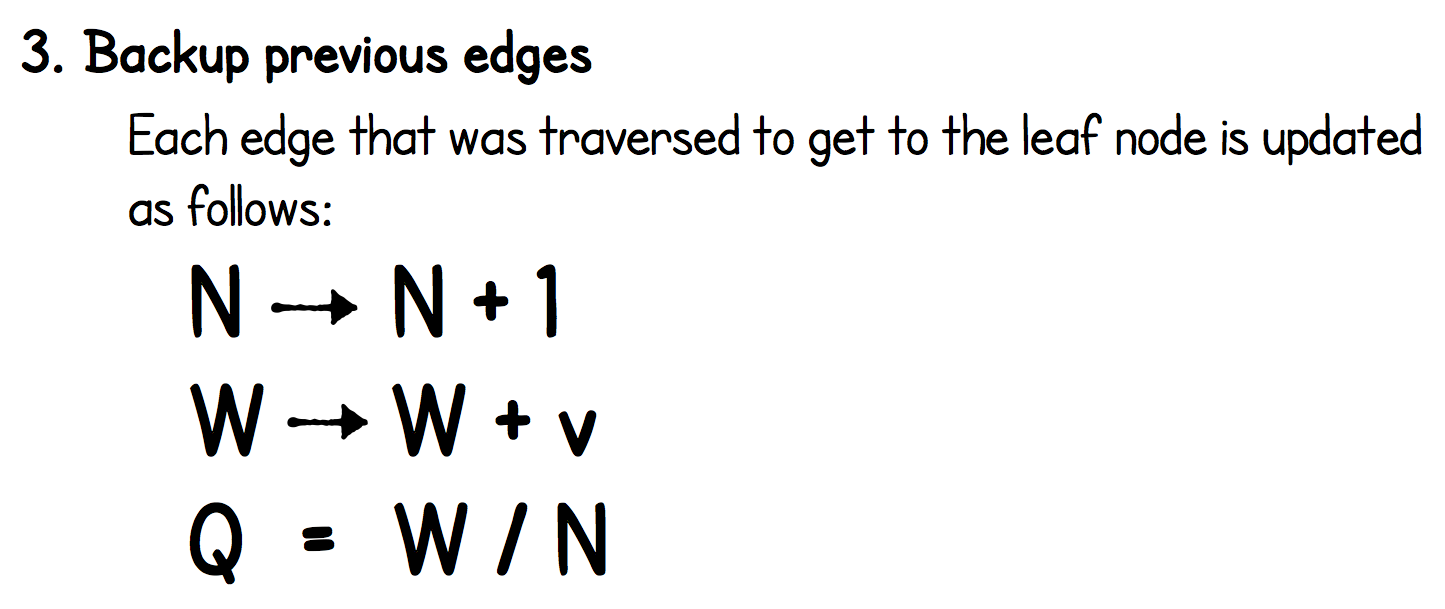
\includegraphics[height=0.5\textheight]{fig/alpha_mcts3.png}
    \end{figure}
\end{frame}

\begin{frame}
    \frametitle{How AlphaGo Zero Chooses Its Next Move}

    \begin{figure}
        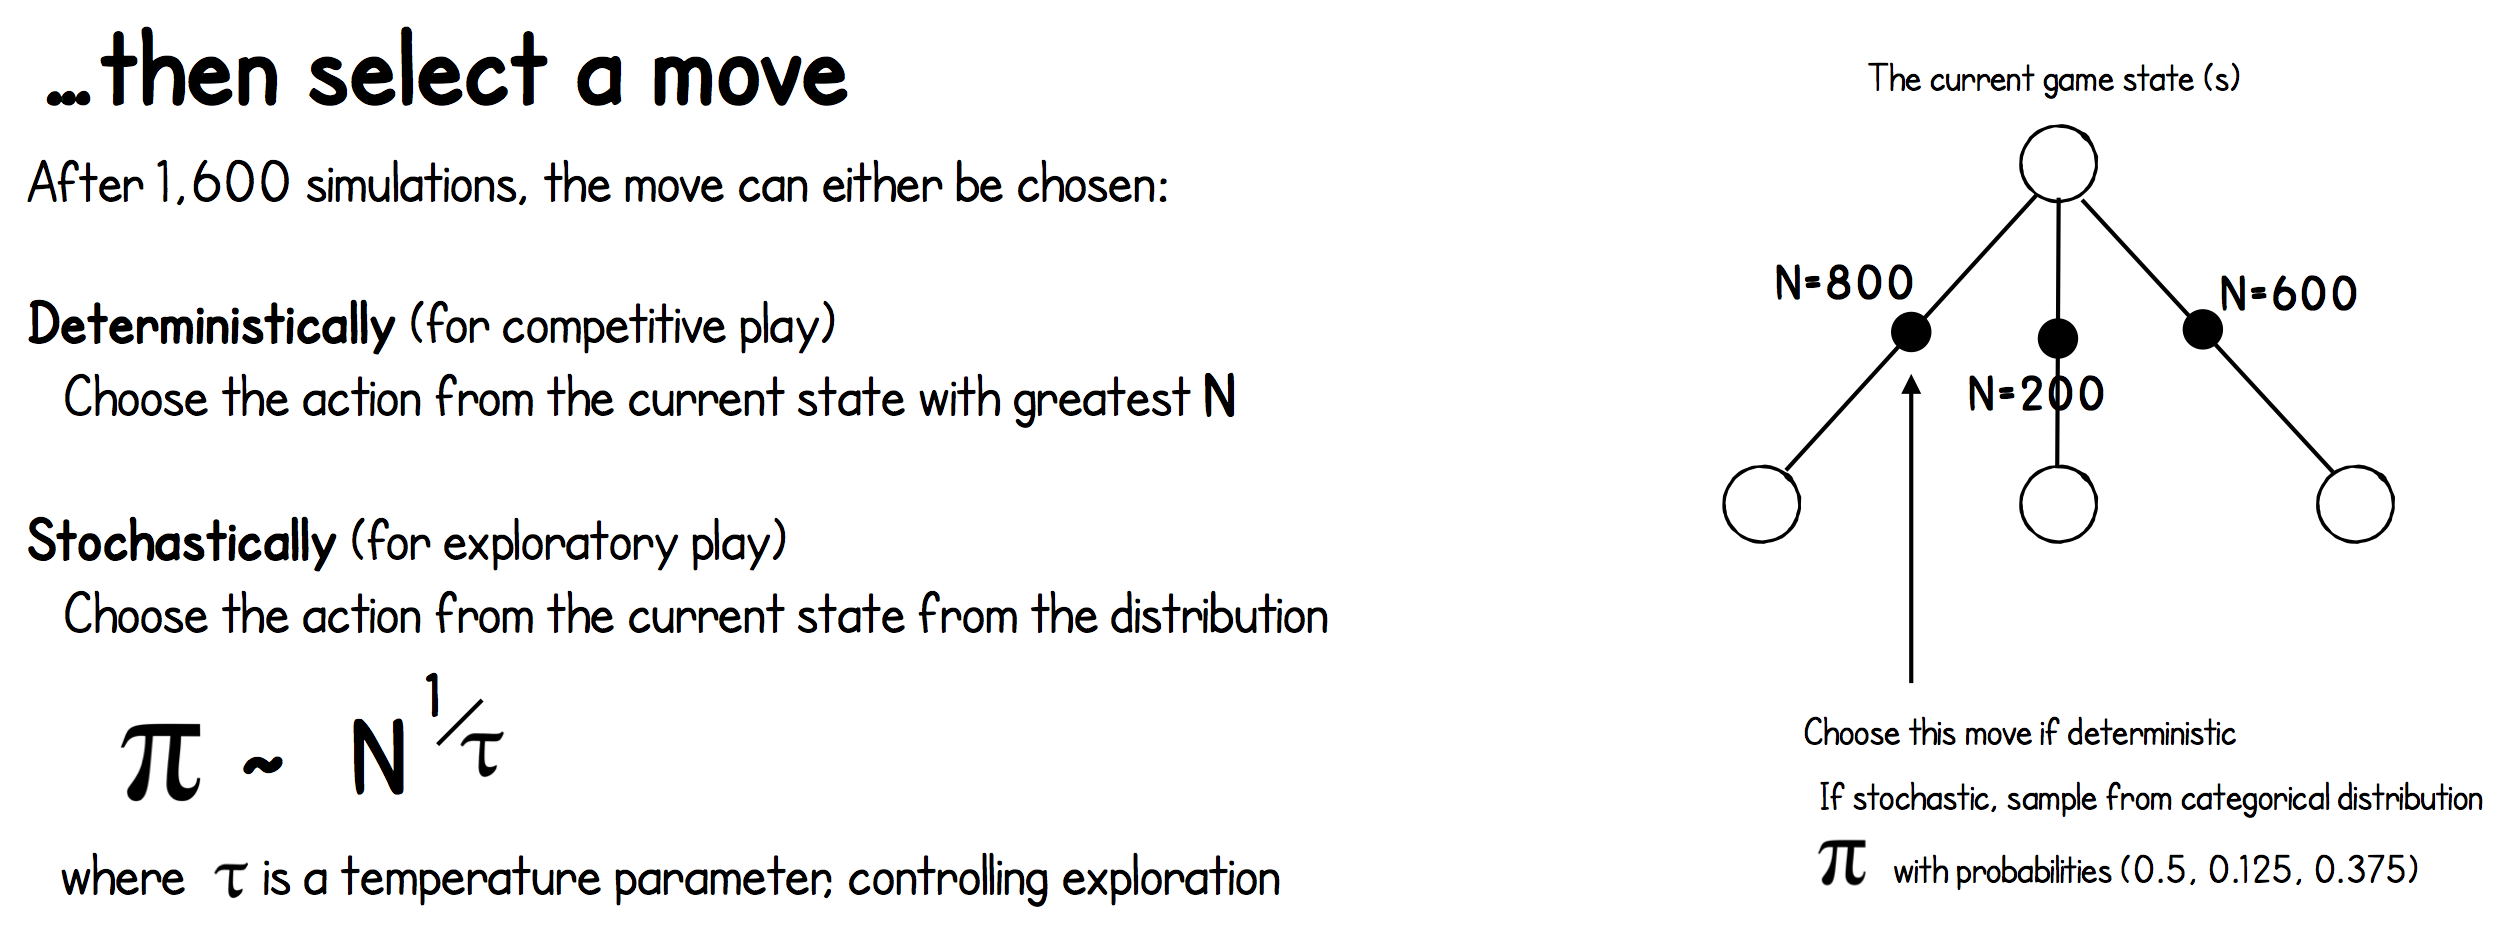
\includegraphics[width=\textwidth]{fig/alpha_mcts4.png}
    \end{figure}
\end{frame}

\begin{frame}
    \frametitle{Self Play}

    \begin{figure}
        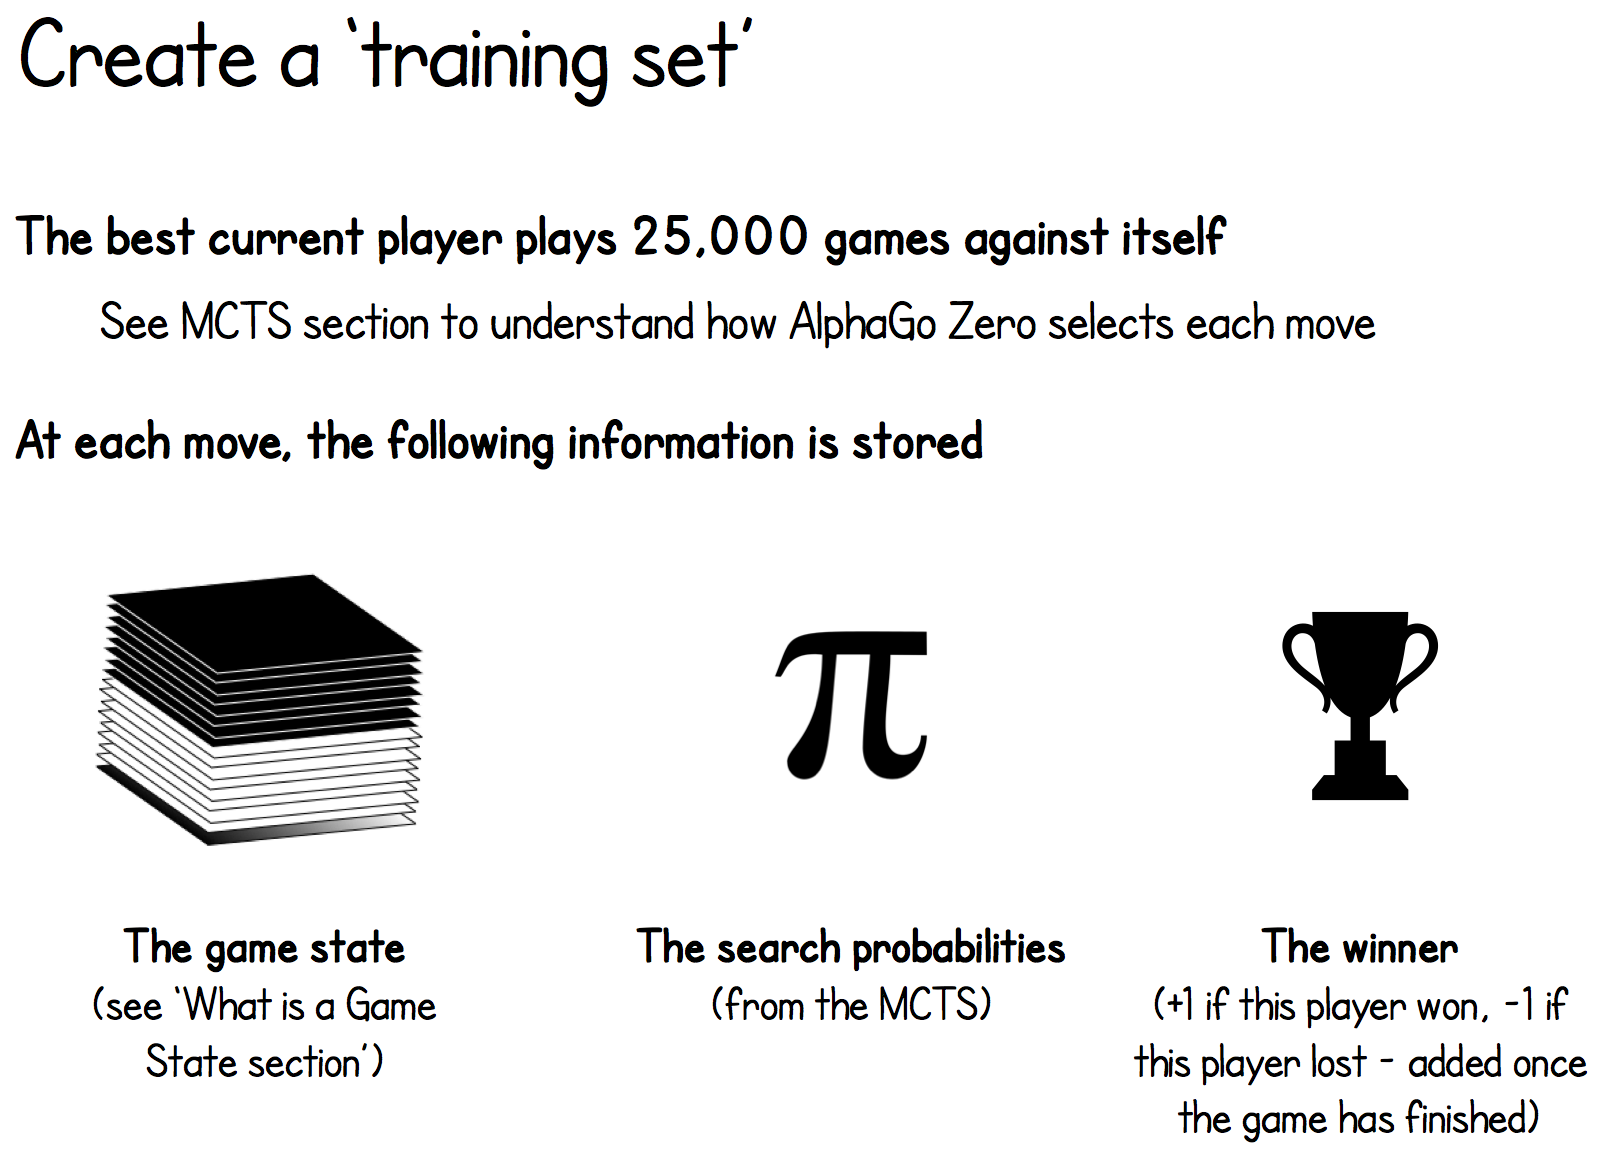
\includegraphics[width=0.9\textwidth]{fig/self_play.png}
    \end{figure}
\end{frame}

\begin{frame}
    \frametitle{Retrain Network}

    \begin{figure}
        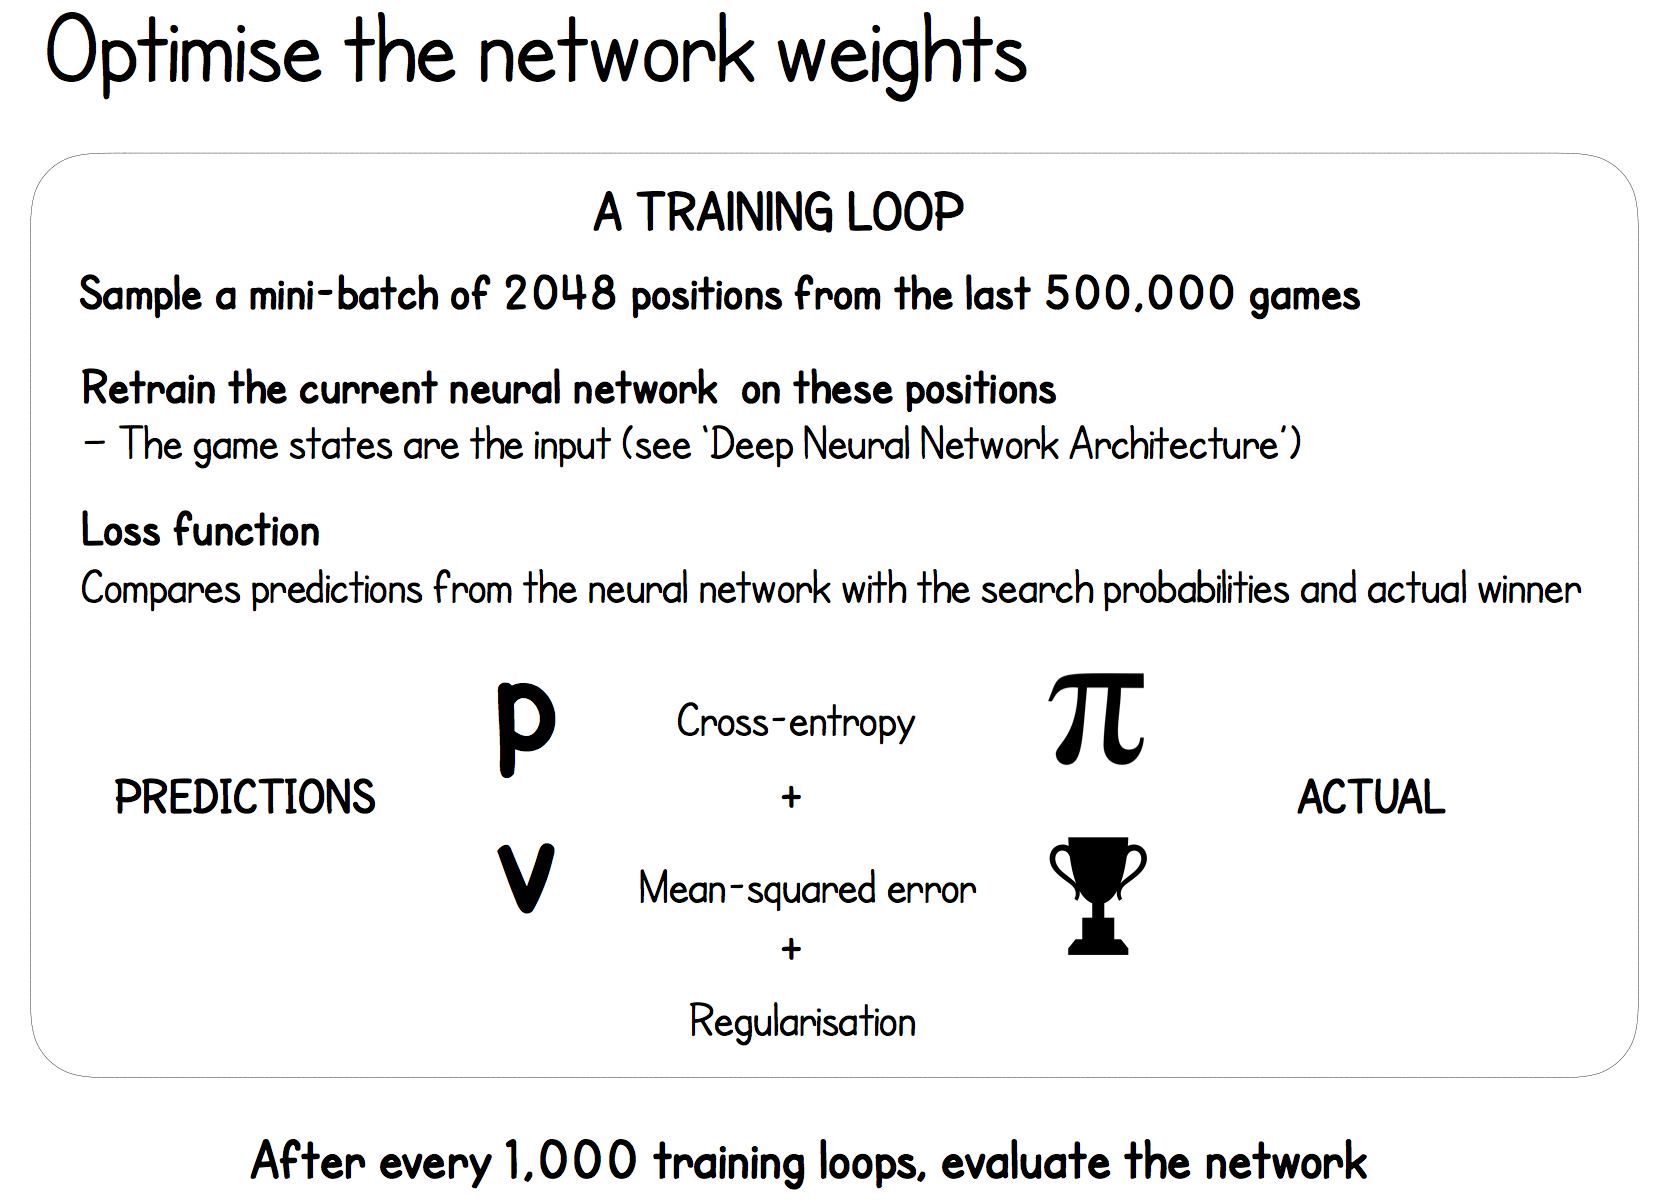
\includegraphics[width=0.9\textwidth]{fig/retrain_network.png}
    \end{figure}
\end{frame}

\begin{frame}
    \frametitle{Reinforcement Learning}

    \begin{figure}
        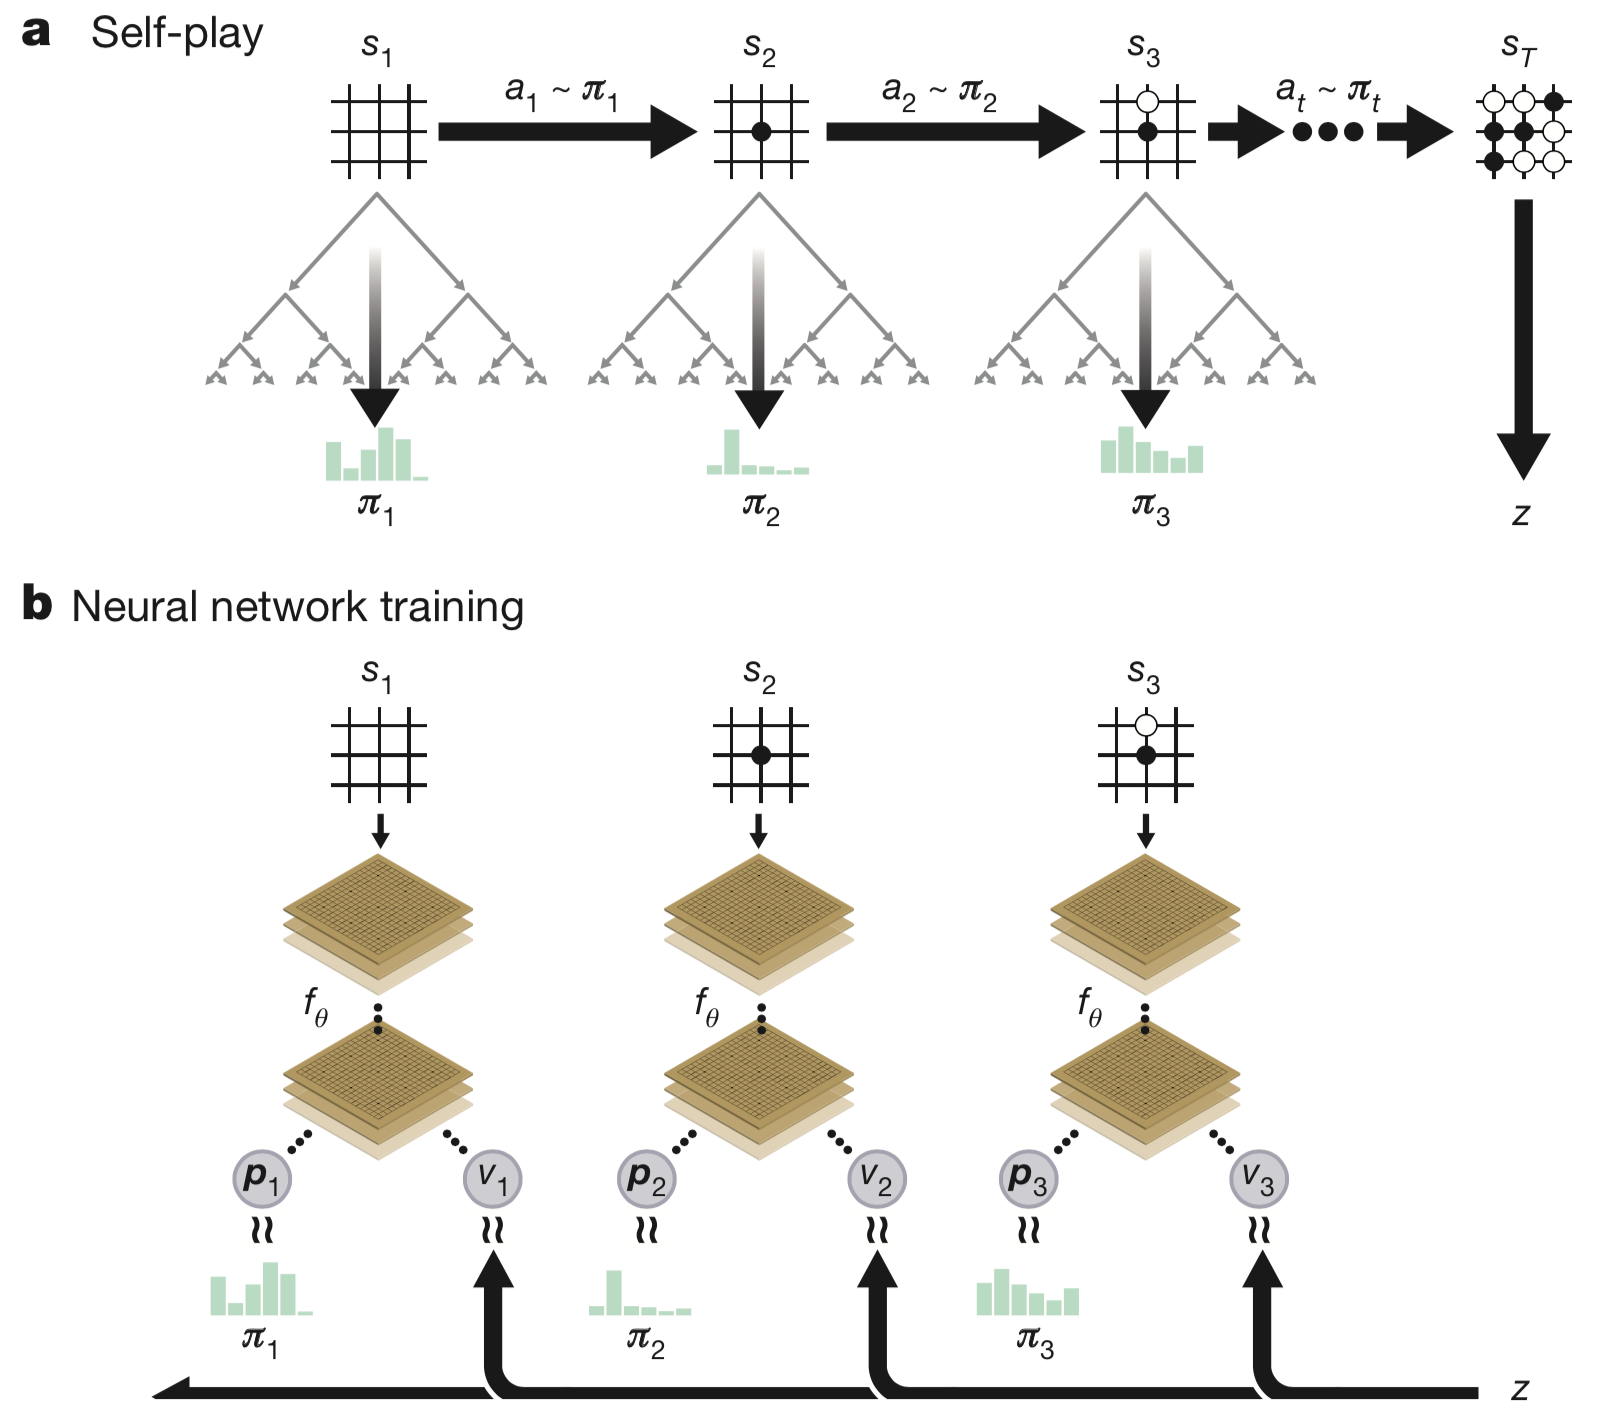
\includegraphics[width=0.75\textwidth]{fig/reinforcement_learning.png}
    \end{figure}
\end{frame}

\begin{frame}
    \frametitle{Evaluate Network}

    \begin{figure}
        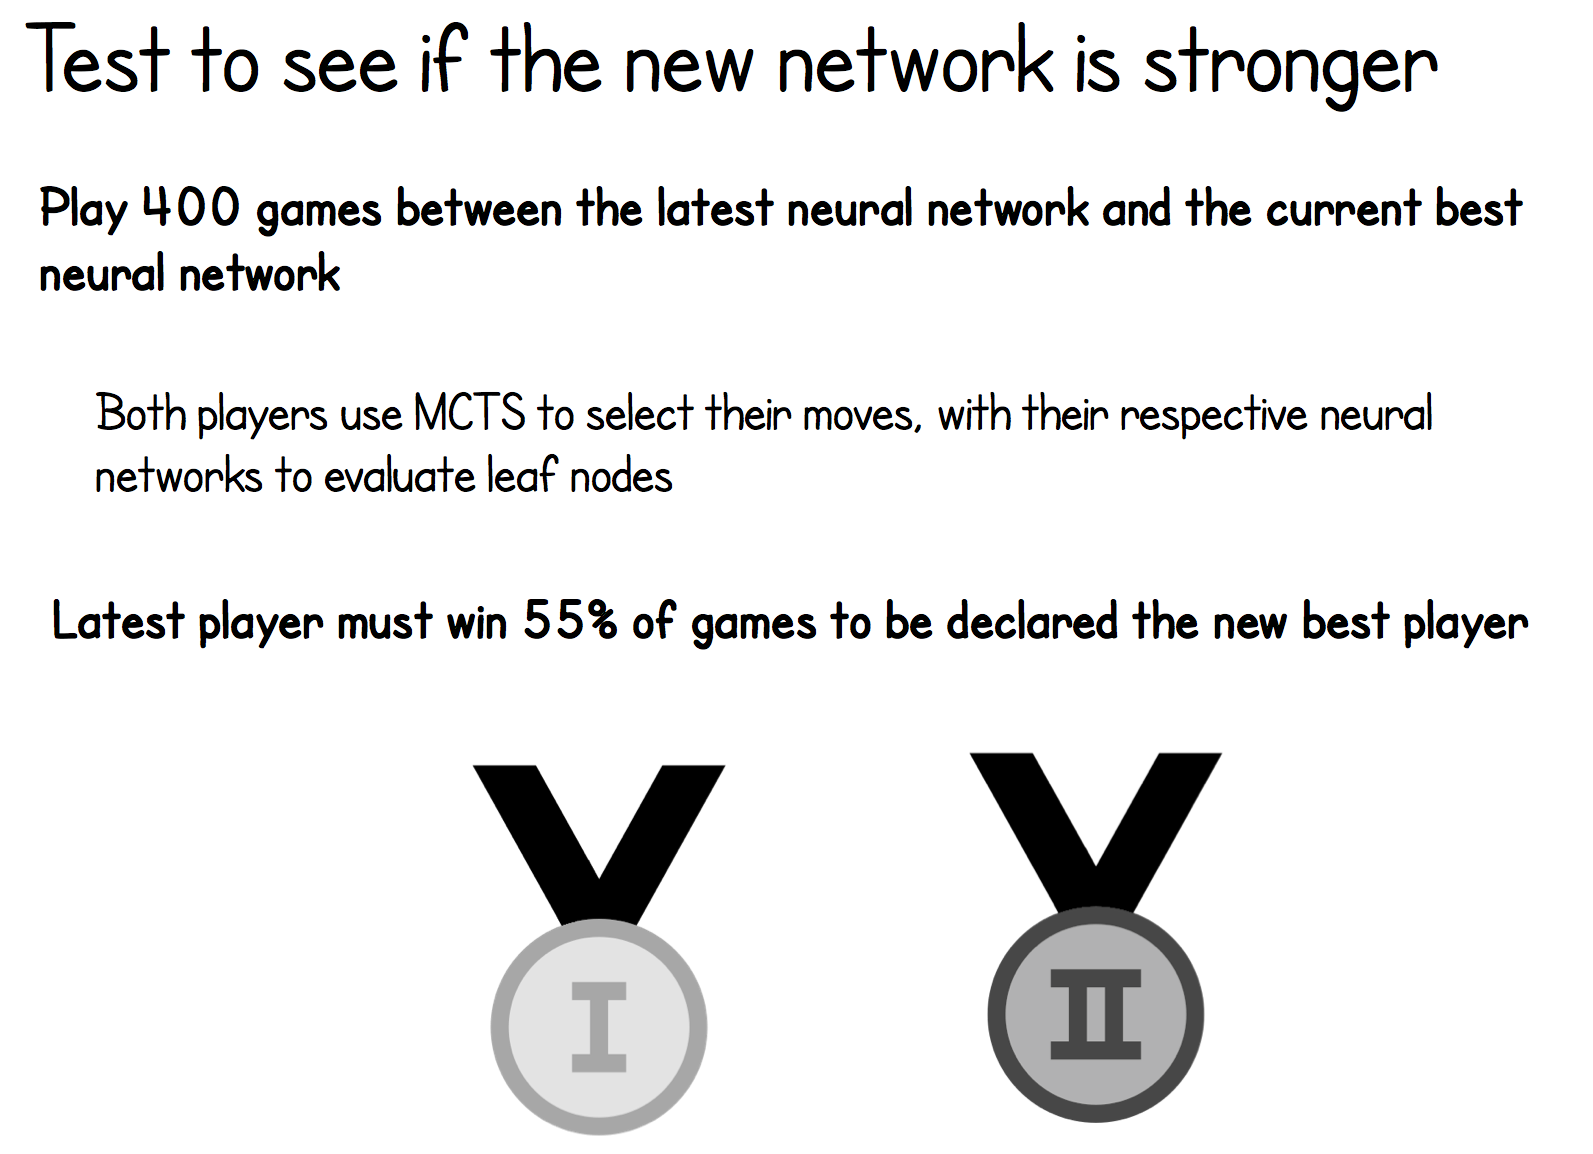
\includegraphics[width=0.85\textwidth]{fig/evaluate_network.png}
    \end{figure}
\end{frame}

\section{Rubiks Cube}
\begin{frame}
    \center \huge \textbf{Rubiks Cube Problem}
\end{frame}

\begin{frame}
    \frametitle{Rubik's Cube}

    \begin{columns}
        \begin{column}{0.5\textwidth}
            \begin{itemize}
            \reditem The 3x3x3 Rubik's cube is a classic 3-Dimensional combination puzzle
            \reditem 6 faces, or 3x3x1 planes, which can be rotated $90^\circ$ in either direction
            \reditem The goal state is reached when all stickers on each face of the cube are the same color
            \end{itemize}
        \end{column}

        \begin{column}{0.5\textwidth}
        \begin{figure}
            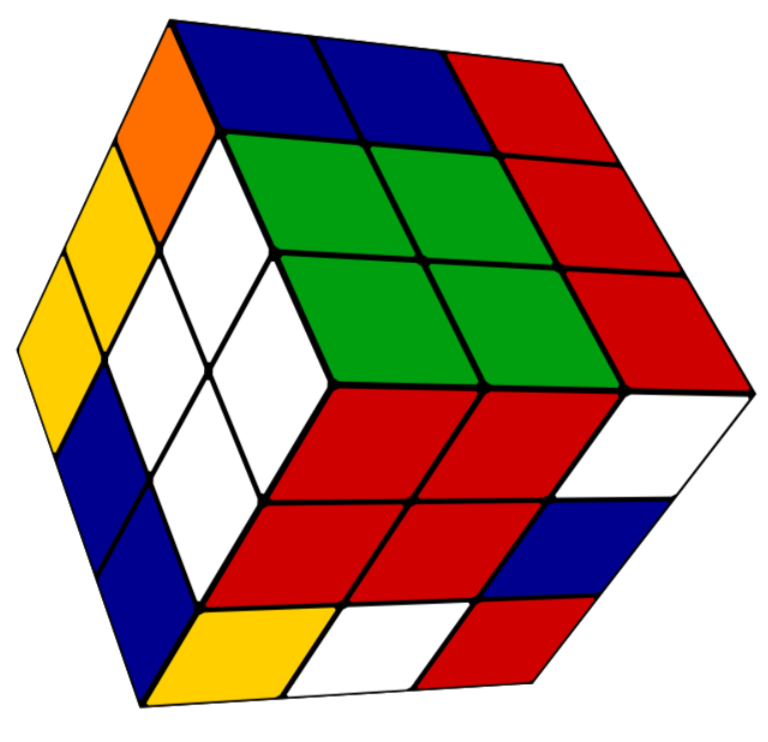
\includegraphics[width=0.8\textwidth]{fig/rubiks_cube.png}
            \caption{3x3x3 Rubik's cube}
        \end{figure}
        \end{column}
    \end{columns}
\end{frame}


\begin{frame}
    \frametitle{Problems}

    \begin{itemize}
        \reditem Large state space \\
        With approximately $4.3x10^{19}$ different possible configurations

        \reditem Single one reward state \\
        Out of all of these configurations, only one state has a reward signal: the goal state
    \end{itemize}

    \begin{columns}
    \begin{column}{.9\textwidth}
    \begin{block}{Difficulties}
        Current DRL(deep reinforcement learning) algorithms struggle in environments with a high number of states and \underline{a small number of reward states}.
        \\[1em]
        Starting from random states and applying DRL algorithms, such as asynchronous advantage actor-critic (A3C), could theoretically result in the agent never solving the cube and never receiving a learning signal.
    \end{block}
    \end{column}
    \end{columns}
\end{frame}

\begin{frame}
    \frametitle{States}

    \begin{itemize}
    \reditem[-] The Rubik’s Cube consists of 26 smaller cubes called cubelets
    \reditem[-] These are classified by their sticker count
    \reditem[-] One-hot encoding for the 54 stickers to represent their location on the cube
    \end{itemize}

    \begin{figure}
        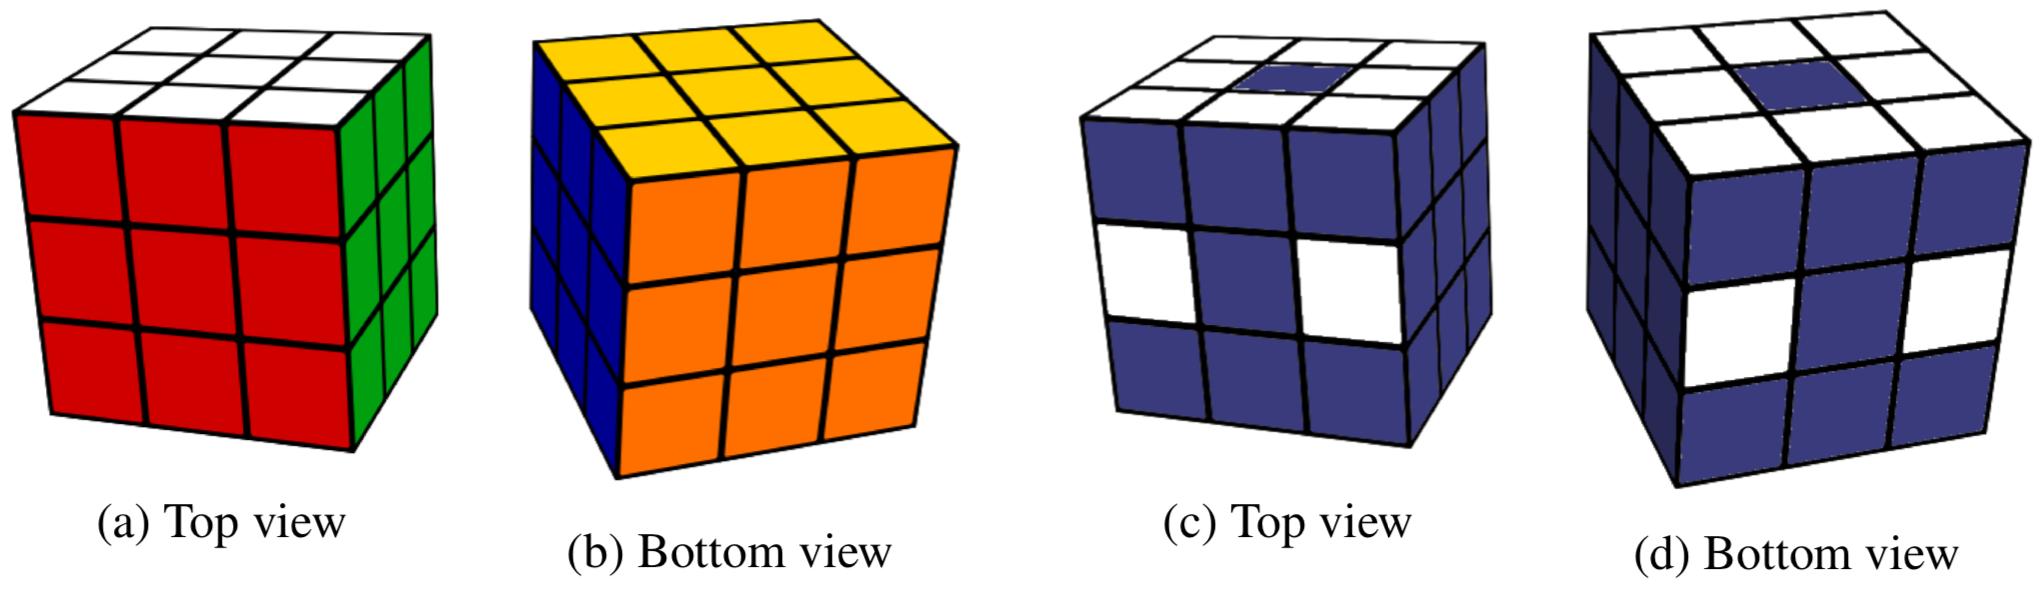
\includegraphics[width=0.9\textwidth]{fig/rubiks_cube_state.png}
        \caption{(a) and (b) show the solved cube as it appears in the environment. (c) and (d) show the cube reduced in dimensionality for input into the DNN. Stickers that are used by the DNN are white, whereas ignored stickers are dark.}
    \end{figure}

\end{frame}

\begin{frame}
    \frametitle{States}

    \begin{itemize}
    \reditem[-] The position of one sticker on a cubelet determines the position of the remaining stickers on that cubelet
    \reditem[-] Ignore the redundant center cubelets and only store the 24 possible locations for the edge and corner cubelets
    \end{itemize}

    \begin{columns}

    \begin{column}{.1\textwidth}\end{column}
    \begin{column}{.4\textwidth}
        \begin{figure}
            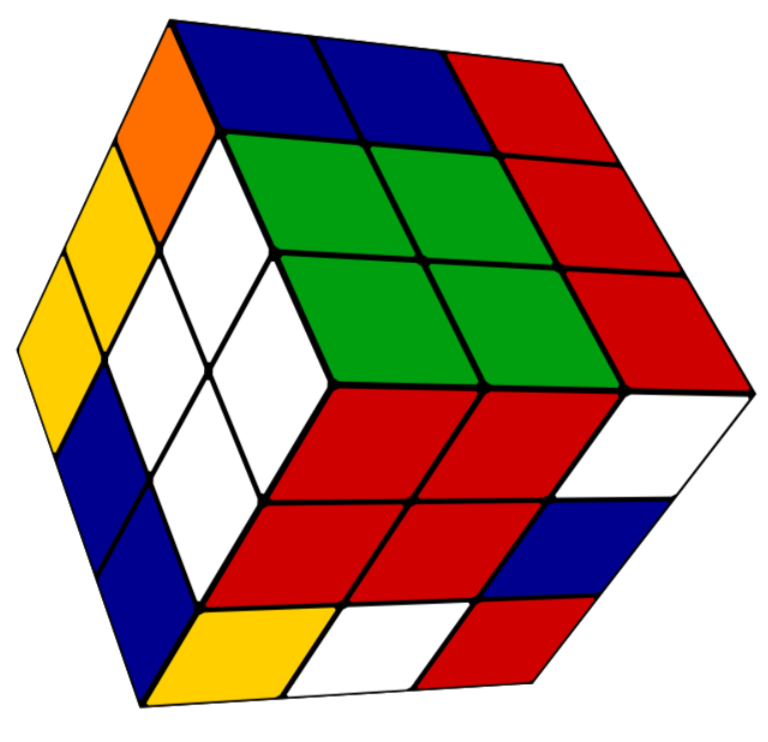
\includegraphics[width=0.8\textwidth]{fig/rubiks_cube.png}
        \end{figure}
    \end{column}

    \begin{column}{.5\textwidth}
        \Large
        \begin{align*}
        \longrightarrow \quad 20 \left[
                \begin{matrix}
                0 & 1 & \cdots & 0 \\
                0 & 0 & \cdots & 1 \\
                \vdots & \vdots & \ddots & \vdots \\
                1 & 0 & \cdots & 0 \\
                \end{matrix}
             \right] \\
        24 \quad\quad &
        \end{align*}
    \end{column}
    \begin{column}{.1\textwidth}\end{column}

    \end{columns}

    \center \large 20x24 State Representation

\end{frame}

\begin{frame}
    \frametitle{Actions}

    F, B, L, R, U, and D correspond to turning the front, back, left, right, up, and down faces.
    \\[1em]
    A clockwise rotation is represented with a single letter, whereas a letter followed by an apostrophe represents a counter-clockwise rotation.

    \begin{figure}
        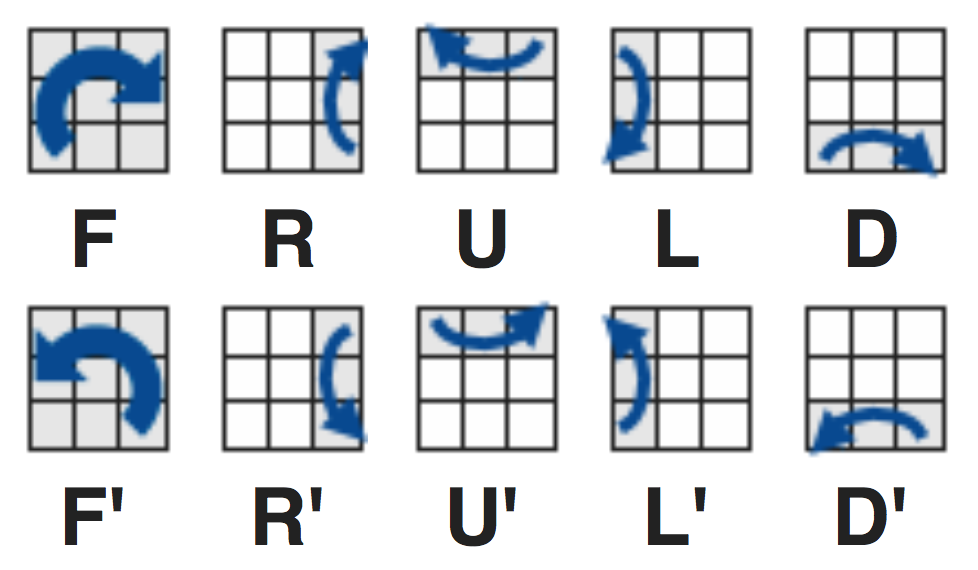
\includegraphics[width=0.6\textwidth]{fig/rubiks_cube_action.png}
        \caption{Moves notation}
    \end{figure}

\end{frame}

\begin{frame}
    \frametitle{Model environment}

    The Rubik's Cube environment consists of
    \begin{itemize}
    \reditem A set of $4.3x10^{19}$ states $\cal{S}$
    \reditem One special state, $s_{solved}$, representing the goal state
    \reditem At each timestep, $t$, the agent
        \begin{itemize}
            \reditem observes a state $s_t \in \cal{S}$
            \reditem takes an action $a_t \in \cal{A}$ with $\cal{A}$ $:= \{F, F', \cdots , D, D'\}$
            \reditem observes a new state $s_{t+1} = A(s_t, a_t)$
            \reditem receives a scalar reward $R(s_{t+1})$, which is $1$ if $s_{t+1}$ is $s_{solved}$ and $-1$ otherwise
        \end{itemize}
    \end{itemize}

\end{frame}

\begin{frame}
    \frametitle{Methods}

    \begin{figure}
        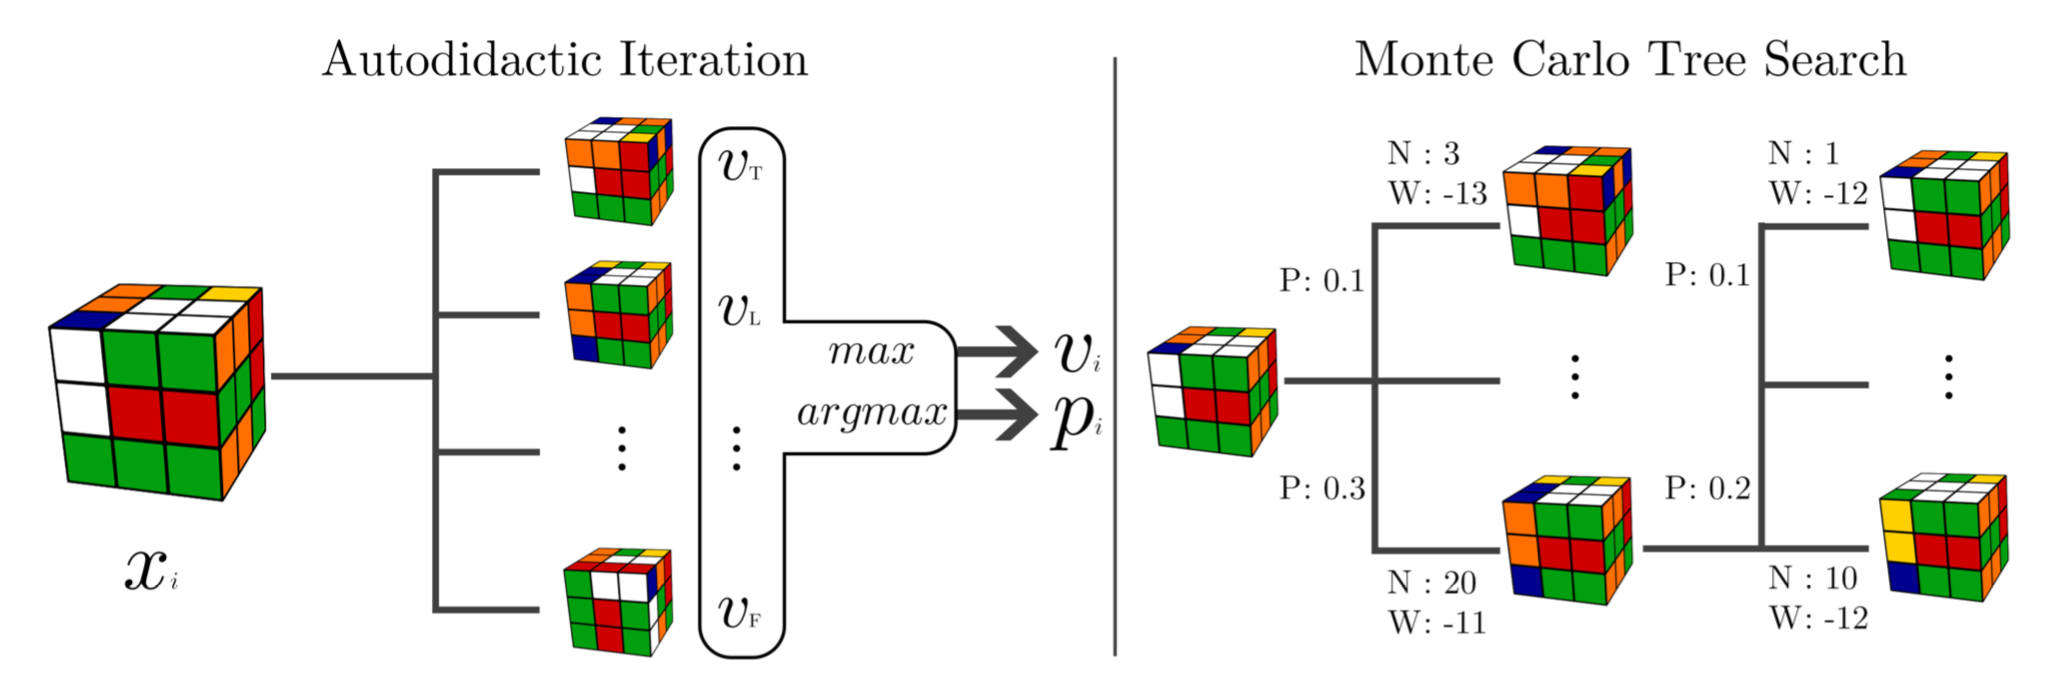
\includegraphics[width=\textwidth]{fig/deepcube_method.png}
        \caption{An illustration of DeepCube. The training and solving process is split up into ADI and MCTS. First, iteratively train a DNN by estimating the true value of the input states using breadth-first search. Then, using the DNN to guide exploration, solve cubes using Monte Carlo Tree Search.}
    \end{figure}
\end{frame}

\begin{frame}
    \frametitle{Autodidactic Iteration} % 自学迭代

    \begin{figure}
        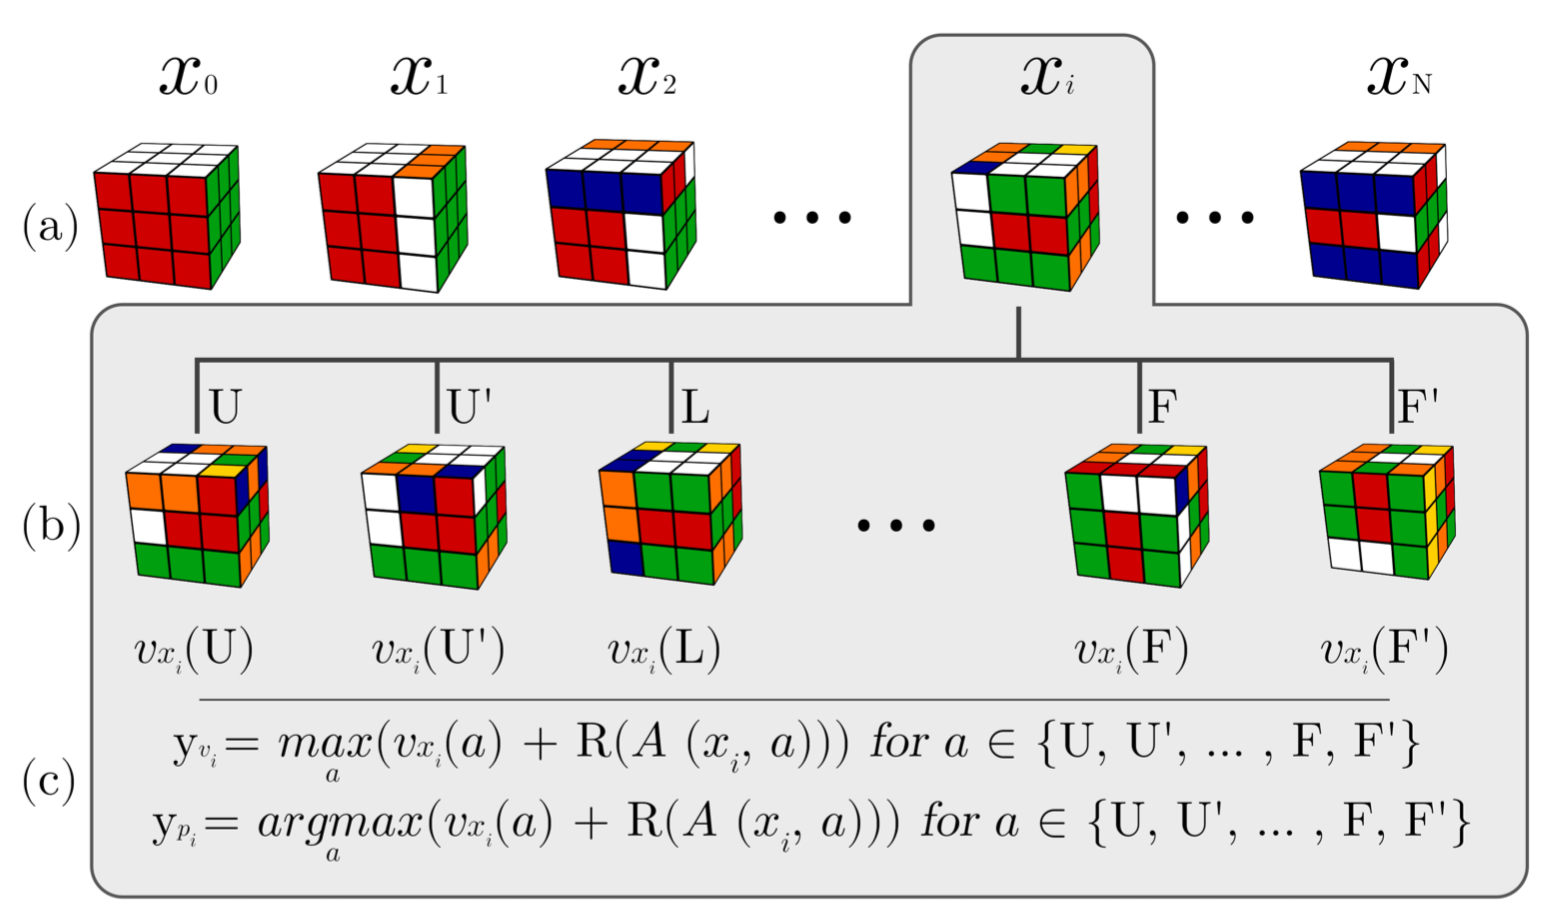
\includegraphics[width=.8\textwidth]{fig/autodidactic_iteration.png}
        \caption{Visualization of training set generation in ADI. (a) Generate a sequence of training inputs starting from the solved state. (b) For each training input, generate its children and evaluate the value network on all of them. (c) Set the value and policy targets based on the maximal estimated value of the children.}
    \end{figure}
\end{frame}

\begin{frame}
    \frametitle{Autodidactic Iteration}

    \normalem % 去掉条件的下划线
    \begin{algorithm}[H]
    \SetKwInOut{Init}{Initialization}
    \DontPrintSemicolon
    \caption{Autodidactic Iteration}
    \Init{$\theta$ initialized using Glorot initialization}
    \Repeat{$iterations = M$}{
        $X$ $\leftarrow$ N scrambled cubes \;
        \For{$x_i \in X$}{
          \For{$\alpha \in \cal{A}$}{
                $(v_{x_i}(\alpha), p_{x_i}(\alpha)) \leftarrow f_{\theta}(A(x_i, \alpha))$
            }
            $y_{v_i} \leftarrow \mathop{\max}_{\alpha}(R(A(x_i, \alpha)) + v_{x_i}(\alpha))$ \;
            $y_{p_i} \leftarrow \mathop{\arg\max}_{\alpha}(R(A(x_i, \alpha)) + v_{x_i}(\alpha))$ \;
            $Y_i \leftarrow (y_{v_i}, y_{p_i})$
        }
        $\theta^{'} \leftarrow train(f_{\theta}, X, Y)$ \;
        $\theta \leftarrow \theta^{'}$
    }
    \end{algorithm}
\end{frame}

\begin{frame}
    \frametitle{MCTS Solver}

    \scriptsize
    \normalem
    \begin{algorithm}[H]
    \DontPrintSemicolon
    \caption{MCTS Solver}
    \KwIn{a starting state $s_0$}
    \KwOut{shortest path from $s_0$ to $s_{solve}$}

    \Repeat{$s_{\tau} = s_{solve} \; \mathbf{or} \; iterations = limit$}{
        \While{$s_t$ is not leaf node}{
            $U_{s_t}(\alpha) \leftarrow cP_{s_t} \sqrt{\sum_{\alpha^{'}}N_{s_t}(\alpha^{'})} / (1 + N_{s_t}(\alpha))$  \tcc*[r]{Select}
            $Q_{s_t}(\alpha) \leftarrow W_{s_t}(\alpha) - L_{s_t}(\alpha)$ \;
            $A_t \leftarrow \mathop{\arg\max}_{\alpha} U_{s_t}(\alpha) + Q_{s_t}(\alpha)$ \;
            $s_t \leftarrow A(s_t, A_t)$
        }
        $s_{\tau} \leftarrow s_t$ \;
        \ForEach{child $s^{'} \in \{A(s_{\tau},\alpha), \forall \alpha \in \cal{A} \}$}{
            $W_{s^{'}}(\cdot), N_{s^{'}}(\cdot), L_{s^{'}}(\cdot) \leftarrow 0$  \tcc*[r]{Expand}
            $P_{s^{'}}(\cdot) \leftarrow p_{s^{'}}$
        }
        $(v_{s_{\tau}}, p_{s_{\tau}}) \leftarrow f_{\theta}(s_{\tau})$ \;
        \For{$t=\tau$ \emph{\KwTo} $0$}{
            $W_{s_t}(A_t) \leftarrow \max(W_{s_t}(A_t), v_{s_{\tau}})$  \tcc*[r]{Backpropagate}
            $N_{s_t}(A_t) \leftarrow N_{s_t}(A_t) + 1$ \;
            $L_{s_t}(A_t) \leftarrow L_{s_t}(A_t) - \nu$ \;
        }
    }
    \Return $Path = \{ A_t | 0 \le t \le \tau \} \leftarrow BFS(T)$
    \end{algorithm}

\end{frame}

\begin{frame}
    \frametitle{Nueral network architecture}

    \begin{figure}
        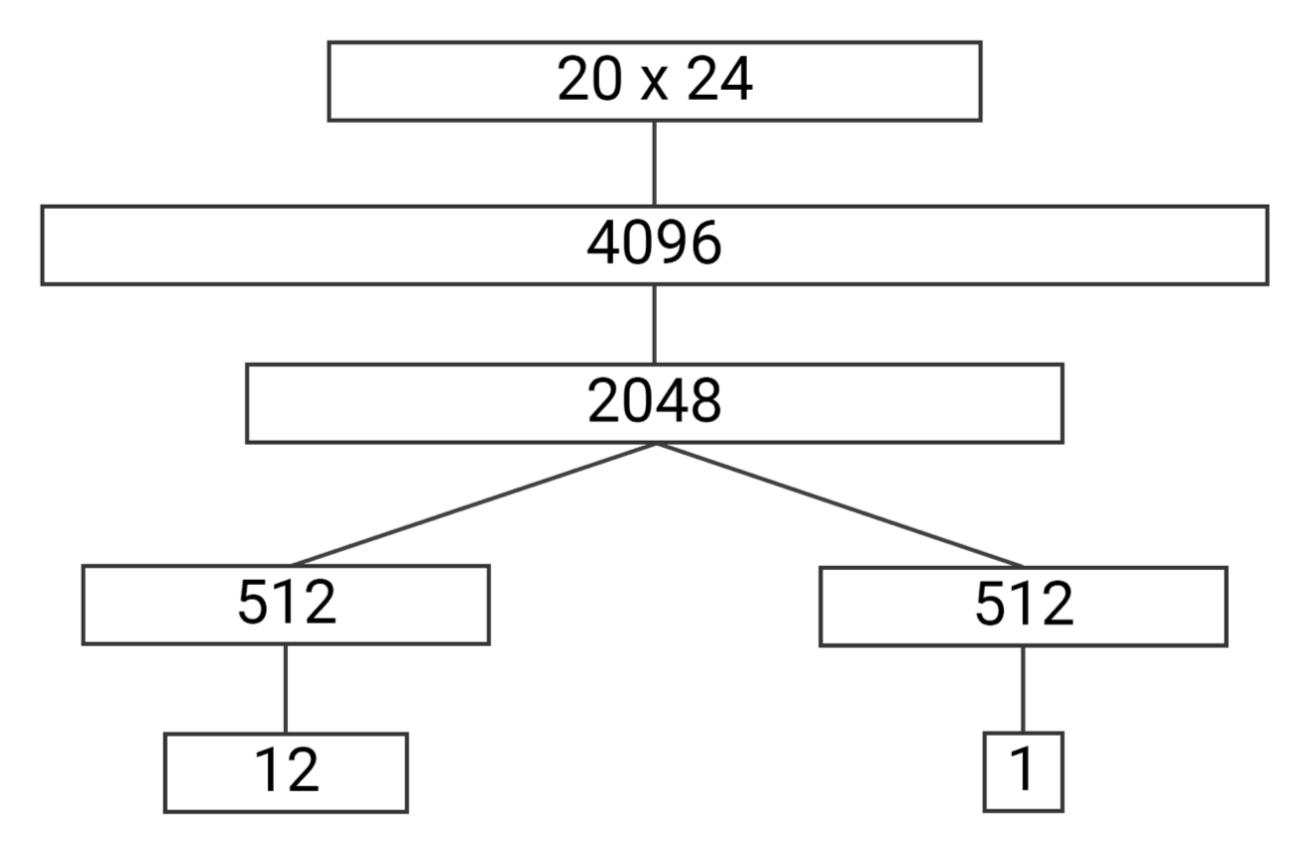
\includegraphics[width=.8\textwidth]{fig/deepcube_nn.png}
        \caption{Architecture for $f_{\theta}$. Each layer is fully connected. Using elu activation on all layers except for the outputs. A combined value and policy network results in more efficient training compared to separate networks.}
    \end{figure}
\end{frame}


\section{Discussion}
\begin{frame}
    \center \huge \textbf{Discussion}
\end{frame}

\begin{frame}
    \frametitle{Discussion}

    \begin{quotation}
    \noindent \huge \textbf{``}

    \normalsize Many combinatorial optimization problems can be thought of as sequential decision making problems, in which case we can use reinforcement learning.
    \\[1.5em]
    Besides further work with the Rubik’s Cube, we are working on extending this method to find approximate solutions to other combinatorial optimization problems such as \color{red} prediction of protein tertiary structure\color{black}.

    \noindent \hspace{24em} \huge \textbf{''}
    \end{quotation}
\end{frame}

\begin{frame}
    \frametitle{Protein folding}

    \begin{quotation}
    \noindent \huge \textbf{``}

    \normalsize For example, in protein folding, we can think of sequentially placing each amino acid in a 3D lattice at each timestep. If we have a model of the environment, ADI can be used to train a value function which looks at a partially completed state and predicts the future reward when finished. This value function can then be combined with MCTS to find approximately optimal conformations.

    \noindent \hspace{24em} \huge \textbf{''}
    \end{quotation}
\end{frame}

\begin{frame}
    \frametitle{Some thoughts on RNA structure predition}

    \begin{figure}
        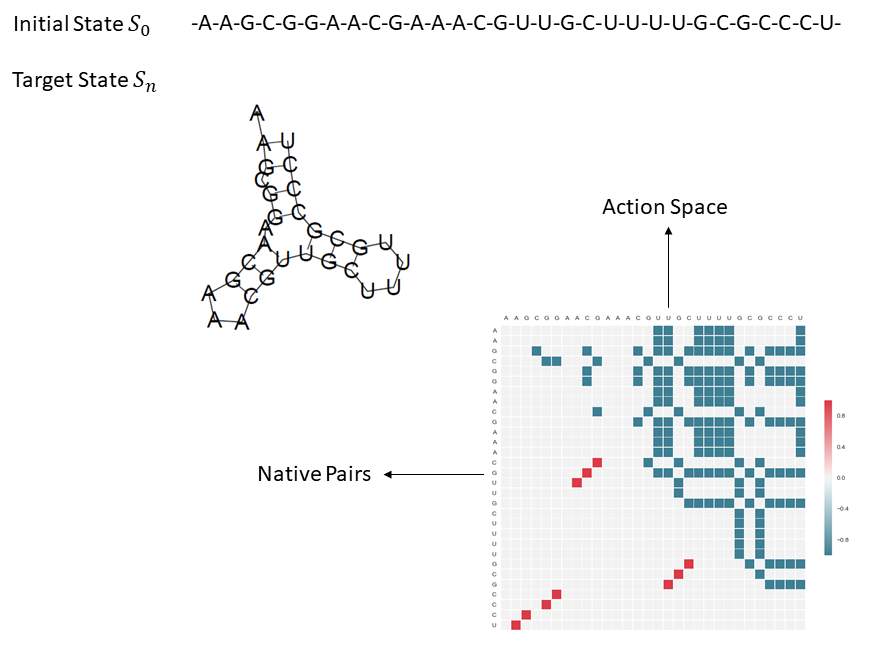
\includegraphics[height=0.85\textheight]{fig/rna_folding1.png}
    \end{figure}
\end{frame}

\begin{frame}
    \frametitle{State evaluation function}

    \begin{figure}
        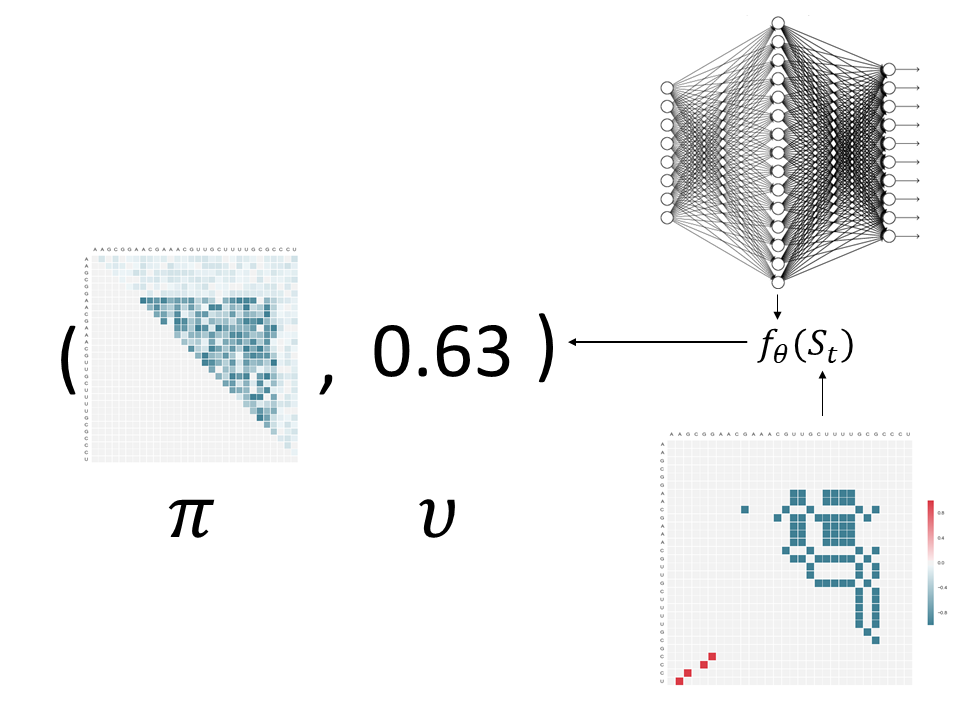
\includegraphics[height=0.9\textheight]{fig/rna_folding2.png}
    \end{figure}
\end{frame}

\begin{frame}
    \frametitle{MCTS to find optimal conformation}

    \begin{figure}
        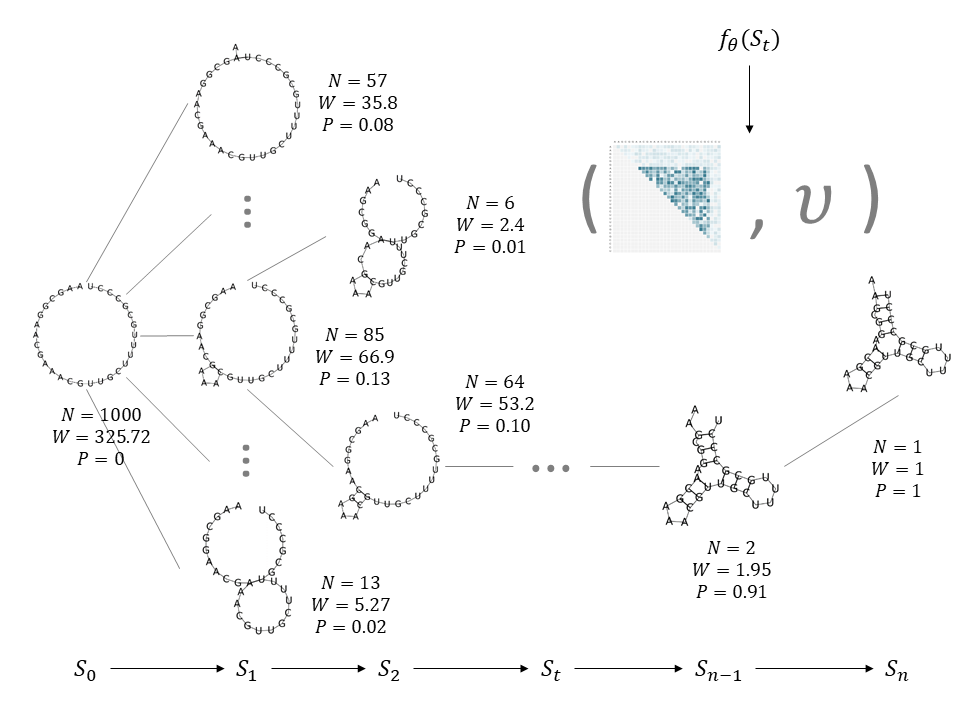
\includegraphics[height=0.9\textheight]{fig/rna_folding3.png}
    \end{figure}
\end{frame}

\begin{frame}
    \frametitle{Deep insight into AlphaGo Zero}

    \begin{columns}
        \begin{column}{.6\textwidth}
            \begin{figure}
                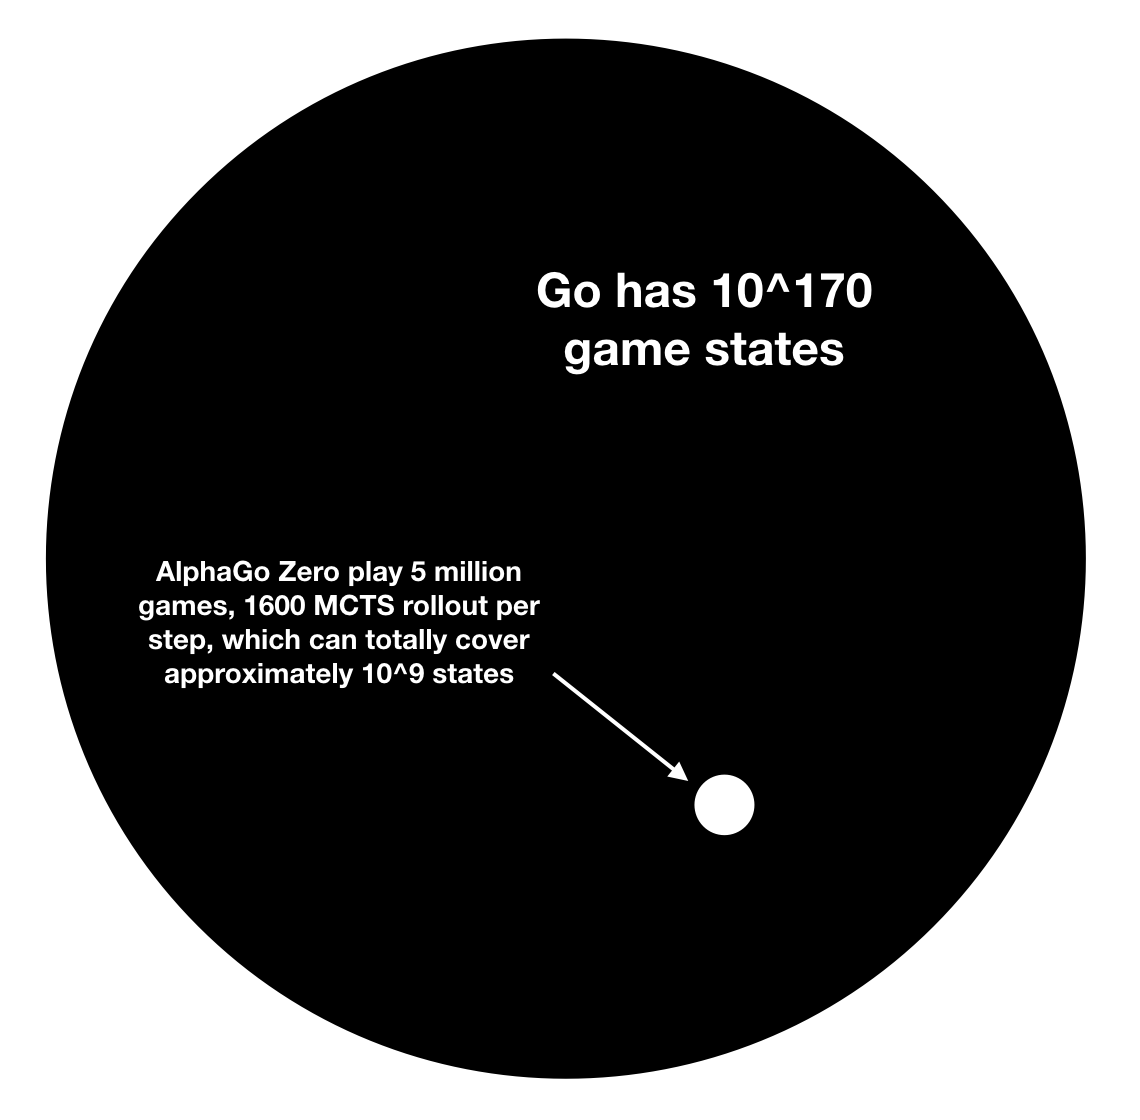
\includegraphics[width=\textwidth]{fig/go_state_space.png}
            \end{figure}
        \end{column}
        \begin{column}{.4\textwidth}
            Previous methods also using self-play and MCTS but not well, maybe the key point is CNN.
        \end{column}
    \end{columns}
\end{frame}


\section{END}
\begin{frame}
    \center \huge \textbf{End}
\end{frame}

\subsection{References}
\begin{frame}
    \frametitle{References}

    \begin{itemize}
        \reditem AlphaGo Zero - How and Why it Works \\
                \url{http://tim.hibal.org/blog/alpha-zero-how-and-why-it-works/}

        \reditem Alpha Go Zero Cheat Sheet \\
                \url{https://applied-data.science/static/main/res/alpha_go_zero_cheat_sheet.png}

        \reditem Mastering the game of Go with deep neural networks and tree search \\
                \url{https://deepmind.com/research/publications/mastering-game-go-deep-neural-networks-tree-search/}

        \reditem Mastering the game of Go without Human Knowledge \\
                \url{https://deepmind.com/research/publications/mastering-game-go-without-human-knowledge/}

        \reditem Solving the Rubik’s Cube Without Human Knowledge \\
                \url{https://arxiv.org/pdf/1805.07470v1.pdf}
    \end{itemize}
\end{frame}


\end{document}